%%%%%%%%%%%%%%%%%%%%%%%%%%%%%%%%%%%%%%%%%%%%%%%%%%%%%%%%%%%%%%%%%%%%%%%%%%%%%%%%
%%%%%%%%%%%%%%%%%%   Vorlage für eine Abschlussarbeit   %%%%%%%%%%%%%%%%%%%%%%%%
%%%%%%%%%%%%%%%%%%%%%%%%%%%%%%%%%%%%%%%%%%%%%%%%%%%%%%%%%%%%%%%%%%%%%%%%%%%%%%%%

% Erstellt von Maximilian Nöthe, <maximilian.noethe@tu-dortmund.de>
% ausgelegt für lualatex und Biblatex mit biber

% Kompilieren mit 
% latexmk --lualatex --output-directory=build thesis.tex
% oder einfach mit:
% make

\documentclass[
% tucolor,       % remove for less green,
  BCOR=12mm,     % 12mm binding corrections, adjust to fit your binding
  parskip=half,  % new paragraphs start with half line vertical space
  open=any,      % chapters start on both odd and even pages
  cleardoublepage=plain,  % no header/footer on blank pages
]{tudothesis}
\renewcommand*{\chapterheadstartvskip}{\vspace*{.5\baselineskip}}
%\chapterheadstartvskip
% Warning, if another latex run is needed
\usepackage[aux]{rerunfilecheck}

% just list chapters and sections in the toc, not subsections or smaller
\setcounter{tocdepth}{1}

%------------------------------------------------------------------------------
%------------------------------ Fonts, Unicode, Language ----------------------
%------------------------------------------------------------------------------
\usepackage{fontspec}
\defaultfontfeatures{Ligatures=TeX}  % -- becomes en-dash etc.

% german language
\usepackage{polyglossia}
\setdefaultlanguage{german}

% for english abstract and english titles in the toc
\setotherlanguages{english}

% intelligent quotation marks, language and nesting sensitive
\usepackage[autostyle]{csquotes}

% microtypographical features, makes the text look nicer on the small scale
\usepackage{microtype}

%------------------------------------------------------------------------------
%------------------------ Math Packages and settings --------------------------
%------------------------------------------------------------------------------

\usepackage{amsmath}
\usepackage{amssymb}
\usepackage{mathtools}

% Enable Unicode-Math and follow the ISO-Standards for typesetting math
\usepackage[
  math-style=ISO,
  bold-style=ISO,
  sans-style=italic,
  nabla=upright,
  partial=upright,
]{unicode-math}
\setmathfont{Latin Modern Math}

% nice, small fracs for the text with \sfrac{}{}
\usepackage{xfrac}  


%------------------------------------------------------------------------------
%---------------------------- Numbers and Units -------------------------------
%------------------------------------------------------------------------------

\usepackage[
  locale=DE,
  separate-uncertainty=true,
  per-mode=symbol-or-fraction,
]{siunitx}
\sisetup{math-micro=\text{µ},text-micro=µ}

%------------------------------------------------------------------------------
%-------------------------------- tables  -------------------------------------
%------------------------------------------------------------------------------

\usepackage{booktabs}       % \toprule, \midrule, \bottomrule, etc

%------------------------------------------------------------------------------
%-------------------------------- graphics -------------------------------------
%------------------------------------------------------------------------------

\usepackage{graphicx}
% currently broken
% \usepackage{grffile}

\usepackage{sidecap}

% allow figures to be placed in the running text by default:
\usepackage{scrhack}
\usepackage{float}
\floatplacement{figure}{htbp}
\floatplacement{table}{htbp}

% keep figures and tables in the section
\usepackage[section, below]{placeins}


%------------------------------------------------------------------------------
%---------------------- customize list environments ---------------------------
%------------------------------------------------------------------------------

\usepackage{enumitem}
\usepackage{pdfpages}
%------------------------------------------------------------------------------
%------------------------------ Bibliographie ---------------------------------
%------------------------------------------------------------------------------

\usepackage[
  backend=biber,   % use modern biber backend
  autolang=hyphen, % load hyphenation rules for if language of bibentry is not
  sorting=none               % german, has to be loaded with \setotherlanguages
                   % in the references.bib use langid={en} for english sources
]{biblatex}
\addbibresource{references.bib}  % the bib file to use
\DefineBibliographyStrings{german}{andothers = {{et\,al\adddot}}}  % replace u.a. with et al.


% Last packages, do not change order or insert new packages after these ones
\usepackage[pdfusetitle, unicode, linkbordercolor=tugreen]{hyperref}
\usepackage{bookmark}
\usepackage[shortcuts]{extdash}

%------------------------------------------------------------------------------
%-------------------------    Angaben zur Arbeit   ----------------------------
%------------------------------------------------------------------------------

\author{Mira Sophie Arndt}
\title{Charakterisierung des Wachstums dünner MgO-Filme auf Fe(100)}
\date{2021}
\birthplace{Unna}
\chair{Lehrstuhl für Experimentelle Physik VI}
\division{Fakultät Physik}
\thesisclass{Bachelor of Science}
\submissiondate{17. August 2021}
\firstcorrector{Prof.~Dr.~Mirko Cinchetti}
\secondcorrector{Prof.~Dr.~Markus Betz}
\thesisbetreuer{David~Janas}
\secondthesisbetreuer{Dr.~Giovanni~Zamborlini}


% tu logo on top of the titlepage
\titlehead{\includegraphics[height=1.5cm]{logos/tu-logo.pdf}}

\begin{document}
\frontmatter
%\thispagestyle{empty}
\setcounter{page}{2}
\section*{Hinweise}
Empfohlen wird die Verwendung dieser Vorlage mit der jeweils aktuellsten TeXLive Version (Linux, Windows) bzw. MacTeX Version (MacOS).
Aktuell ist dies TeXLive 2016. Download hier:
\begin{center}
  \ttfamily\url{https://www.tug.org/texlive/}
\end{center}
Bei Verwendung von TexLive Versionen 2014 und älter sollte
die Zeile
\begin{center}
\verb+\RequirePackage{fixltx2e}+ 
\end{center}
als erste Zeile der Präambel noch vor der Dokumentenklasse eingefügt werden.
Dies lädt diverse Bugfixes für LaTeX, die ab TexLive 2015 Standard sind.

Die Vorlage \texttt{thesis.tex} ist für die Kompilierung mit \texttt{lualatex} ausgelegt, mit wenigen Anpassungen kann sie aber auch mit \texttt{pdflatex} oder \texttt{xelatex} verwendet werden. 
Die Dokumentenklasse \texttt{tudothesis.cls} kann mit allen drei Programmen verwednet werden.

Achten Sie auch auf die Kodierung der Quelldateien.
Bei Verwendung von Xe\LaTeX\ oder Lua\LaTeX\ (empfohlen) müssen die
Quelldateien UTF-8 kodiert sein.
Bei Verwendung von pdf\LaTeX\ nutzen Sie die Pakete \texttt{inputenc} und \texttt{fontenc} mit der korrekten Wahl der Kodierungen.

Eine aktuelle Version dieser Vorlage steht unter 
\begin{center}
  \ttfamily\url{https://github.com/maxnoe/tudothesis}
\end{center}
zur Verfügung.

Alle verwendeten Pakete werden im \LaTeX{} Kurs von Pep et al.\ erklärt:
\begin{center}
  \ttfamily\url{http://toolbox.pep-dortmund.org/notes}
\end{center}

Für Rückmeldungen und bei Problemen mit der Klasse oder Vorlage, bitte ein \emph{Issue} auf GitHub aufmachen oder eine Email an
\href{mailto:maximilian.noethe@tu-dortmund.de}{maximilian.noethe@tu-dortmund.de} schreiben.

Wenn Sie die Dokumentenklasse mit der Option \texttt{tucolor} laden, werden verschiedene Elemente in TU-Grün gesetzt.

\maketitle

% Gutachterseite
\makecorrectorpage

% hier beginnt der Vorspann, nummeriert in römischen Zahlen
%\thispagestyle{plain}

\section*{Kurzfassung}
Hier steht eine Kurzfassung der Arbeit in deutscher Sprache inklusive der Zusammenfassung der
Ergebnisse.
Zusammen mit der englischen Zusammenfassung muss sie auf diese Seite passen.

\section*{Abstract}
\begin{english}
The abstract is a short summary of the thesis in English, together with the German summary it has to fit on this page.
\end{english}

\tableofcontents

\mainmatter
% Hier beginnt der Inhalt mit Seite 1 in arabischen Ziffern
\chapter{Einleitung}

Durch die fortschreitende Miniaturisierung technischer Bauteile spielen die 
physikalischen Effekte an Oberflächen und Grenzflächen dünner Schichtsysteme 
eine immer größere Rolle.\newline
In der Vergangenheit wurden im Bereich der Spinelektronik bereits viele relevante Entdeckungen gemacht, deren 
Anwendungen heutzutage in der Industrie weit verbreitet sind.
Als Beispiel kann der gigantische Magnetwiderstand 
aufgeführt werden, zu dessen vielen Anwendungen Spin-Ventile gehören,
welche flächendeckend in Leseköpfen von Computerfestplatten genutzt werden \cite{PhysRevLett.61.2472,PhysRevB.39.4828,daughton2000gmr,jogschies2015recent}. 
Ein verwandter Effekt ist der magnetische Tunnelwiderstand, 
der genutzt wird um magnetische Tunnelkontakte
zu erzeugen \cite{JULLIERE1975225}. Bereits hier wurde die Relevanz von Fe/MgO/Fe-Systemen
wegen ihres großen Tunnelwiderstandes deutlich \cite{parkin2004giant}.\newline
Gegenstand aktueller Forschung sind molekülbasierte Spintronics \cite{cinchetti2017activating},
bei denen neue Spineffekte an der Grenzfläche zwischen anorganischen und molekularen Schichten untersucht werden.
Die Verwendung von Molekülen bringt dabei mehrere Vorteile mit sich, wie zum Beispiel eine 
lange Spin-Relaxationszeit, selbstständige Anordnung und die Möglichkeit, chemische und physikalische Eigenschaften für 
verschiedene Aufgaben anzupassen \cite{cinchetti2009determination,sun2018progress}. 
Zu den Anwendungen gehören beispielsweise organische licht-emittierende Dioden und Photovoltaic Zellen \cite{koch2007organic}.\newline
Der Einfluss von MgO als dielektrische Zwischenschicht in metallisch/organischen Hybridsystemen wurde  2017 bereits von
Hollerer et al. am Beispiel von Ag(100)/Pentacen bzw. Ag(100)/MgO/Pentacen Grenzschichten diskutiert. Durch das Einführen der 
MgO-Zwischenschicht konnte für den Ladungstransfer zwischen Metall und Molekül ein Übergang von fraktionellem hin zu 
ganzzahligem Ladungstransfer beobachtet werden, welcher auf den einsetzenden Tunneleffekt zurückzuführen ist.
Ein ähnlicher Effekt ist bei der Verwendung von Eisen als Substrat denkbar, 
wobei die im ferromagnetischen Eisen vorliegende Spin-Polarisation auch einen einheitlichen,
spinabhängigen Ladungstransfer zur Folge hätte. Dies könnte widerum Anwendung in zukünftigen spinelektronischen Bauteilen  finden.\newline
Die Herstellung dieser Systeme setzt ein Verständnis über das Wachstum der MgO-Schichten voraus.
Zu diesem Zweck wird in dieser Arbeit das MgO-Wachstum auf Fe(100) und Fe(100)-p(1\,x\,1)O
mit oberflächensensitiven Methoden charakterisiert und verglichen.
Mit den gewonnenen Referenzdaten ist es möglich das Wachstum zu reproduzieren,
auch wenn nicht alle hier verwendeten Methoden zur Verfügung stehen.
Eine Untersuchung der Wachstumsschichtdicke erfolgt duch 
reflektierte Elektronenbeugung und Augerelektronenspektroskopie. 
Letztere Methode wird auch genutzt um eine Elementanalyse vorzunehmen und so die Stöchiometrie zu prüfen.
Zudem wird die Oberflächenstruktur durch Elektronenbeugung charakterisiert.

%Die Stöchiometrie wird mittels einer Elementanalyse geprüft und die 
%Oberflächenstruktur durch Elektronenbeugung charakterisiert.
%

%
%Als Beispiel kann der magnetische Tunnelkontakt (magnetic tunnel junction, "MTJ")
%genannt werden, bei dem die Bedeutung von Fe/MgO/Fe-Systemen
%wegen ihres großen Tunnelwiderstandes gezeigt wurde \cite{parkin2004giant}.\newline
%Durch die fortschreitende Miniaturisierung technischer Bauteile spielen die 
%physikalischen Effekte an Oberflächen und Grenzflächen dünner Schichtsysteme 
%eine immer größer Rolle.\newline
%Dabei wurden im Bereich der Spinelektronik bereits viele relevante Entdeckungen gemacht, deren 
%Anwendungen heutzutage in der Industrie weit verbreitet sind.
%Als Beispiel können die beiden spinabhängigen Effekte gigantische Magnetoresistenz (giant magnetoresistance) 
%und magnetische Tunnelwiderstände (tunnel Magnetoresistance) aufgeführt werden, zu deren vielen Anwendungen zum Beispiel Spin-Ventile gehören,
%welche verbreitet bei der Datenspeicherung genutzt werden \cite{daughton2000gmr,jogschies2015recent}. 
%
%Fertig

%So beschreibt ein Modell von Barraud et al. \cite{barraud2010unravelling} etwa, dass die Spin-Polarisation von ferromagnetischen Materialien 
%an der Grenzfläche zu molekularen Schichten durch die Grenzflächenhybridisierung beeinflussst werden kann.


%Bei solch einem molekularem System wurde bereits von Hollerer et al. \cite{hollerer2017charge}
%die Relevanz von MgO als dielektrische Zwischenschicht entdeckt. In solch einem System ist der übergang von einem 
%fraktionellen Ladungstransfer (durch Hybridisierung) ohne MgO-Zwischenschicht zu einem ganzzahligen Ladungstransfer (durch Elektronentunneln)
%mit MgO-Zwischenschicht zu beobachten.
%



%Eisen spielt als Ferromagnet bei Raumtemperatur eine entscheidende Rolle bei 
%spinabhängigigen Effekten \cite{parkin2004giant,yuasa2004giant}.
%So könnte Eisen genutzt werden, um durch Spinpolarisation das Tunneln 
%der Elektronen durch die MgO Zwischenlage und somit den ganzzahligen Ladungstransfer bei einem Fe/MgO/Pentacene-System 
%in Abhängigkeit des Spins zu manipulieren.
%Die starken magnetischen Eigenschaften an der Oberfläche von reinem Eisen 
%können durch Passivierung und das Erzeugen einer (1\,x\,1)-Überstruktur noch verstärkt werden \cite{tange2010electronic}.
%
%Fertig
%Eisen spielt als Ferromagnet bei Raumtemperatur eine entscheidende Rolle bei 
%spinabhängigigen Effekten \cite{parkin2004giant,yuasa2004giant}. Die starken magnetischen Eigenschaften an der Oberfläche von reinem Eisen 
%können durch Passivierung und das Erzeugen einer (1\,x\,1)-Überstruktur noch verstärkt werden \cite{tange2010electronic}.\newline
%Dielektrische Zwischenschichten an metallischen/molekularen Grenzflächen können zur Entkopplung oder als Tunnelbarriere dienen. 
%So wurden bereits die bedeutenden Einflüsse einer dielektrischen MgO-Zwischenschicht 
%im Dreilagensystem Ag/MgO/Pentacene von Hollerer et al. ausgearbeitet \cite{hollerer2017charge}.
%
%Fertig

\chapter{Grundlagen des Systems}
\section{Fe(100), Fe(100)-p(1\,x\,1)O und MgO}

Eisen ist bei Raumtemperatur ferromagnetisch und kristalliert in einer kubisch-raumzentrierten Kristallstruktur 
mit einer Gitterkonstante von $2,87\,\si{\angstrom}$. 
Die Bezeichnung Fe(100) bezieht sich auf die Miller-Indizes ($h\,k\,l$) und gibt die Orientierung der Kristalloberfläche im Raum an.

Bei der Passivierung mit Sauerstoff setzen sich die Sauerstoffionen auf die Muldenplätze der Fe(100)-Struktur und bilden eine (1\,x\,1)-Überstruktur \cite{jona1987re}.
Die chemische Stabilität der Oberfläche erhöht sich auf diese Weise und die magnetischen Eigenschaften werden gleichzeitig verstärkt \cite{tange2010electronic}.

\begin{SCfigure}
    \centering
    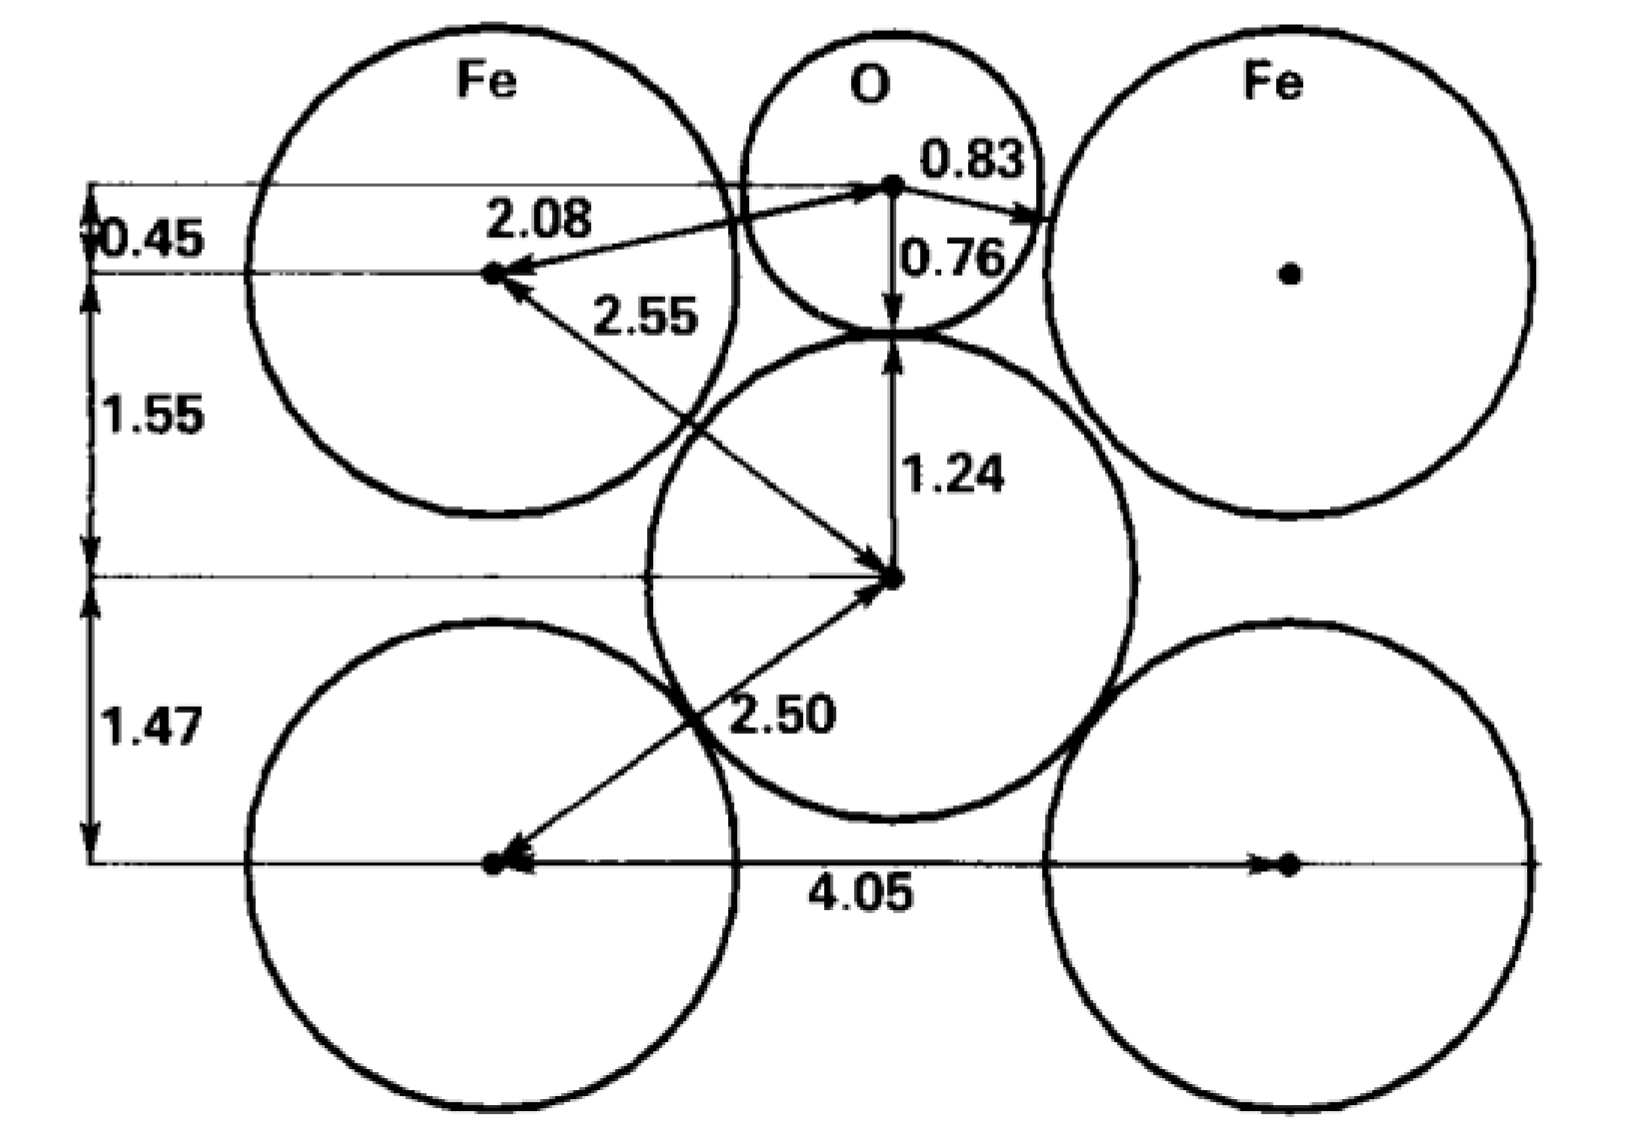
\includegraphics[width=0.45\linewidth]{Plots/FeO_Struktur.png}
    \caption{Schematische Darstellung der Fe(100)-p(1\,x\,1)O-Oberfläche in der Seitenansicht mit Angabe der durch die Passivierung verursachten Deformationen der Fe(100) Oberfläche \cite{jona1987re}.}
    \label{fig:FeO}
\end{SCfigure}

Magnesiumoxid kristallisiert in einer NaCl-Struktur mit einer Gitterkonstante von $4,21\,\si{\angstrom}$.
Eine einzelne Monolage im Festkörper ist demnach $2,105\,\si{\angstrom}$ groß, mit vernachlässigbaren Abweichungen
an der Grenzfläche zu Fe(100)- und Fe(100)-p(1\,x\,1)O-Oberflächen \cite{meyerheim2001geometrical}.




\section{Arten des Schichtwachstums}
\label{sec:Wachstum}

Idealerweise verläuft das Wachstum des Adsorbats lagenweise auf dem Substrat (Frank-van-der-Merwe-Wachstum), sodass Atome erst dann 
eine neue Monolage ("ML") bilden, wenn die vorherige ML vollständig belegt ist.
Ist die Grenzflächenenergie des wachsenden Films zum Substrat und zum Vakuum größer als 
die Energie des Substrats zum Vakuum, so kommt es zu Inselwachstum (Volmer-Weber-Wachstum).
Da es energetisch günstiger ist, möglichst wenig Fläche des Substrats zu bedecken, bildet sich ein Film, der weder einkristallin 
noch von homogener Dicke ist.
Wird dem System Energie in Form von Wärme zugefügt, kann diese Energiedifferenz überwunden werden und bevorzugt ein lagenweises Wachstum 
stattfinden. Die Mischform aus anfänglich lagenweisem Wachstum und anschließendem Inselwachstum wird Stranski-Krastanov-Wachstum genannt \cite{fauster}.

\begin{SCfigure}
    \centering
    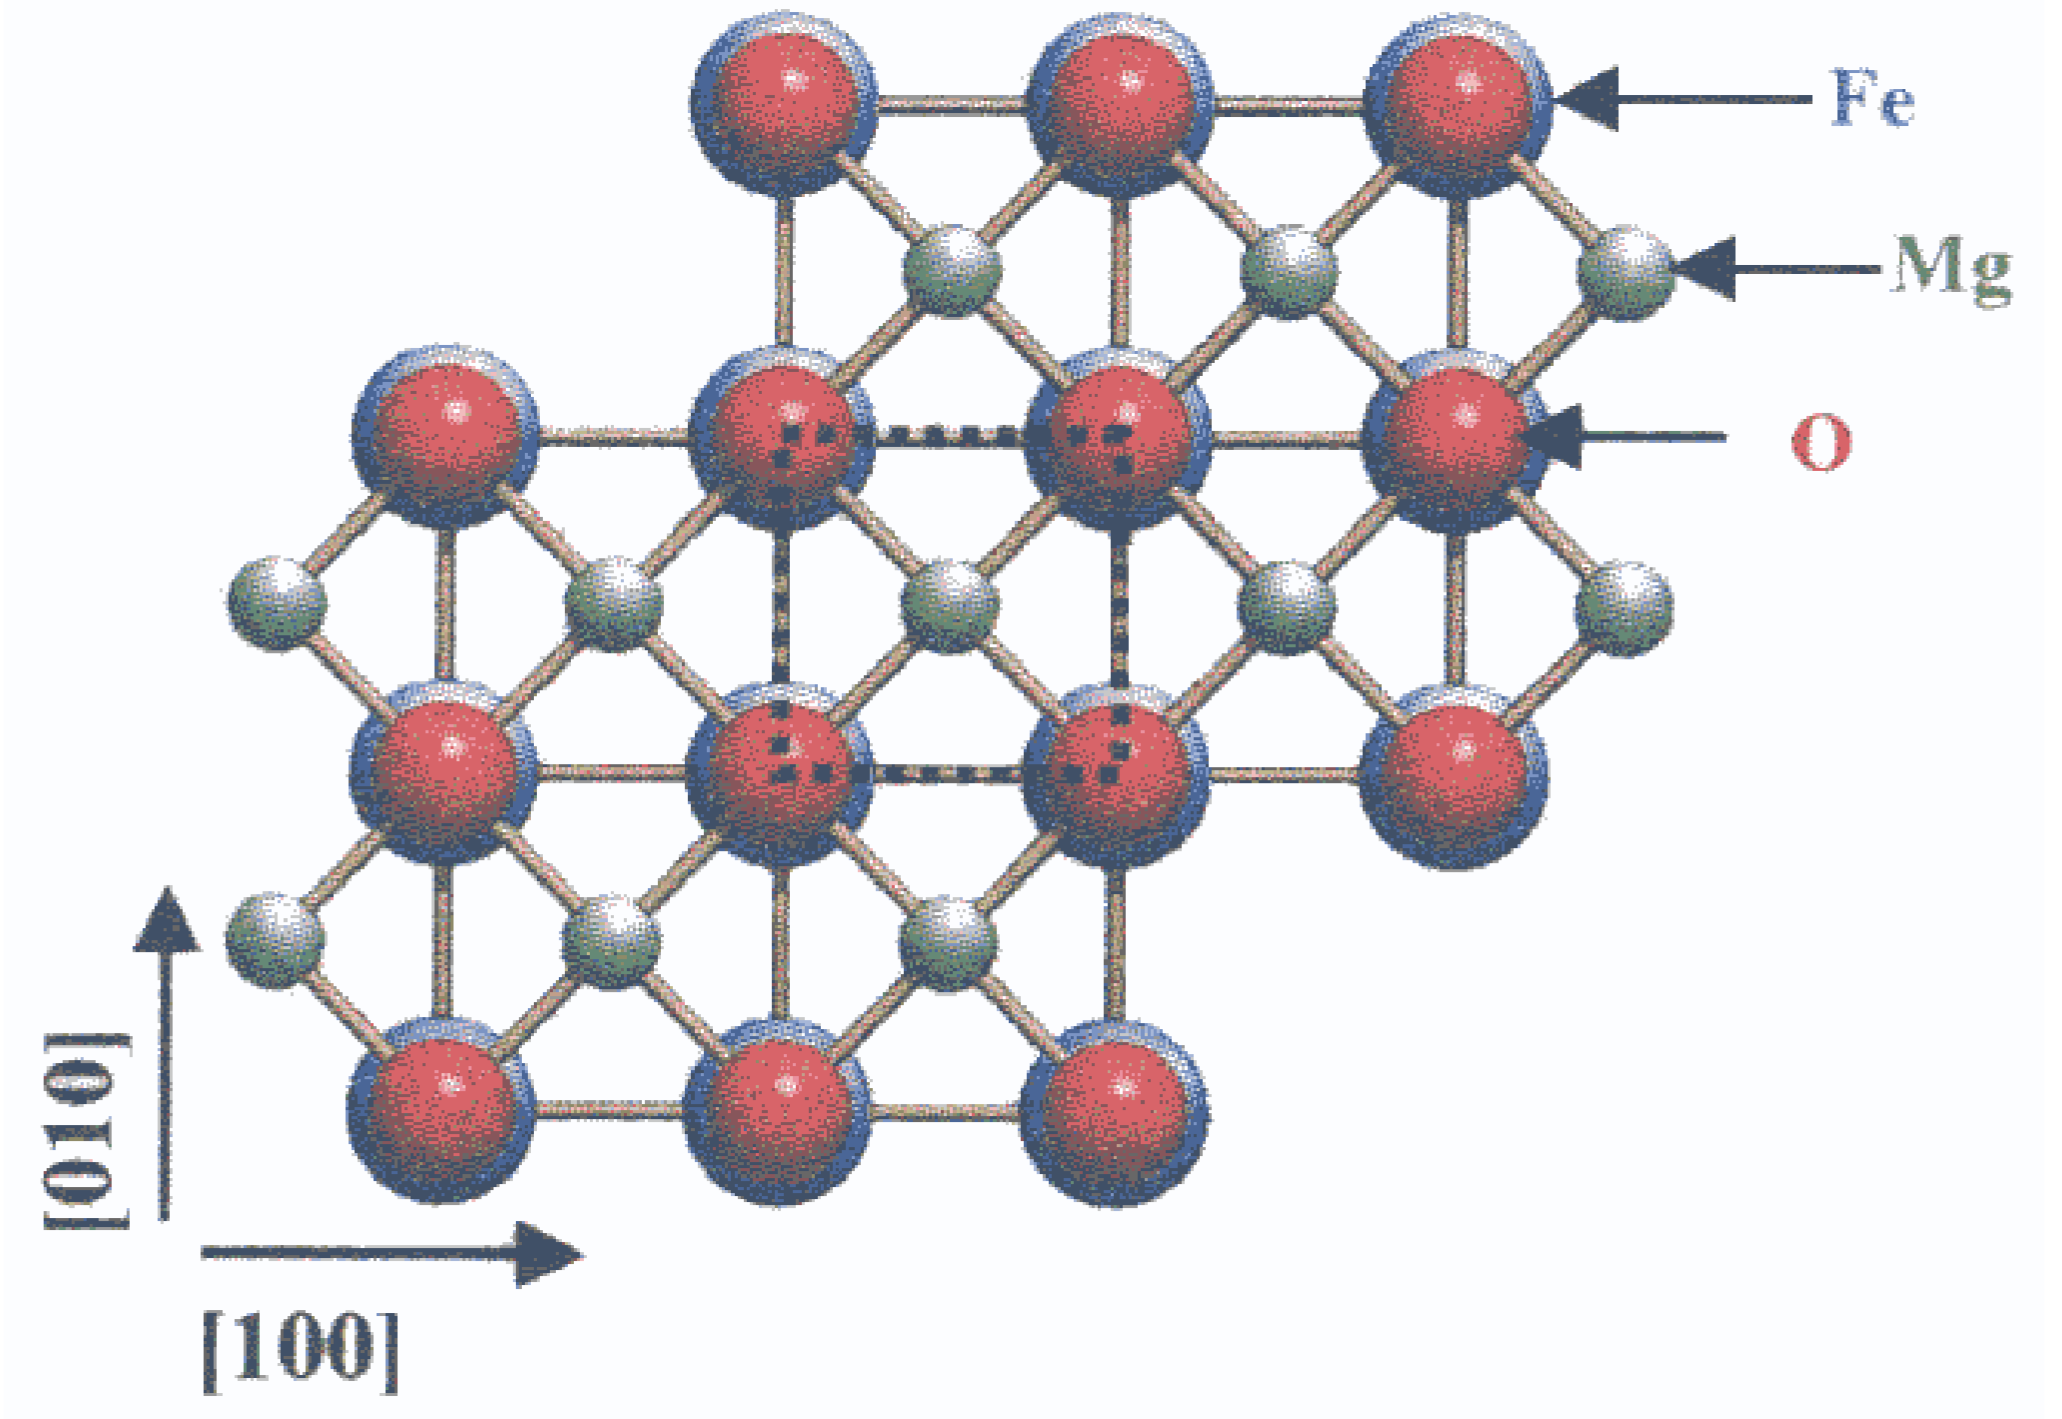
\includegraphics[width=0.45\linewidth]{Plots/Fe_MgO_Struktur.png}
    \caption{Anordnung einer Lage MgO auf Fe(100) in der Draufsicht. Die Sauerstoffionen liegen auf den Eisenatomen, während die Magnesiumionen 
    nach der NaCl-Struktur von MgO zwischen den Sauerstoffplätzen liegen.
    Die Richtungsangaben beziehen sich auf das Fe-System \cite{meyerheim2001geometrical}.}
    \label{fig:Fe_MgO}
\end{SCfigure}

Wenn sowohl Substrat als auch Adsorbat einkristallin sind 
und die wachsende Schicht eine wohldefinierte Beziehung zum Substrat hat, spricht man von Epitaxie.
Beim Wachstum von MgO auf Fe(100) und Fe(100)-p(1\,x\,1)O liegt die [100]-Richtung des Magnesiums in [110]-Richtung 
des Eisens, sodass die Sauerstoffionen auf den Eisenatomen liegen. Es entsteht eine Struktur wie schematisch in Abbildung \ref{fig:Fe_MgO} zu sehen, bei der 
die Gitterkonstante von MgO um $3,7\,\si{\percent}$ vom Atomabstand $\sqrt{2}\cdot 2,87\,\si{\angstrom}=4,06\,\si{\angstrom}$ von Eisen in [110]-Richtung abweicht. 
MgO kann bis zu einer Schichtdicke von 6 ML epitaktisch wachsen \cite{klaua2001growth}, erst danach bilden sich Versetzungen in Folge der 
Fehlanpassung der Gitterkonstanten \cite{dynna1996low}.

Beim Aufdampfen von Mg in einer Sauerstoffatmosphäre kann die Stöchiometrie direkt kontrolliert werden. 
Tekiel et al. \cite{tekiel2013reactive} fanden ein optimiertes Verhältnis der Mg-Aufdampfrate $r$ zum Sauerstoffdruck $p$ von 

\begin{equation}
    \dfrac{r}{p}=(0,15\pm 0,05)\cdot 10^8 \,\si{\angstrom\per\milli\bar\per\minute}.
    \label{eq:V1}
\end{equation}

Auf diese Weise können MgO-Filme mit hoher Stöchiometrie und kristalliner Struktur produziert werden.
\chapter{Methoden}

\section{Quarzkristall-Mikrowaage}
Eine Möglichkeit, die Masse  eines aufgedampften Materials
zu bestimmen, ist die Änderung der Eigenfrequenz 
einer angeregten Quarzplatte (Quartz Crystal Microbalance, "QCM") zu untersuchen.
Durch die Vergrößerung der schwingenden Masse $\symup{\Delta}m$ ändert sich die Frequenz $\symup{\Delta}f$ nach der Sauerbrey Gleichung \cite{sauerbrey1959verwendung},
was auf den linearen Zusammenhang

\begin{equation}
        \symup{\Delta}f = -\symup{C} \cdot \symup{\Delta}m
\end{equation}

führt. Der Faktor $\symup{C}$ bezeichnet eine Kalibrierungskonstante. Aus der aufgedampften Masse lässt sich über die Dichte des Materials 
die gewachsene Schichtdicke und damit die Aufdampfrate in $\si{\angstrom\per\minute}$ bestimmen.
Diese gibt einen Anhaltspunkt für die spätere Aufdampfrate auf der untersuchten Probe, 
weicht aber um einen konstanten Faktor von der tatsächlichen Rate ab. 
Eine Ursache dafür sind unterschiedliche Adsorptionsraten des Quarzkristalls und der untersuchten Probe.




\section{LEED und IV-LEED}

Zur Strukturbestimmung in Festkörpern eignen sich allgemein Beugungsmethoden mit Teilchen, deren Wellenlänge in der Größenordnung der 
zu untersuchenden Struktur liegt. Bei der Beugung niederenergetischer Elektronen (Low Energy Electron Diffraction, "LEED") werden Elektronen 
genutzt, deren Energien im Bereich $E=50$-$200$\,eV liegen, sodass sie zum Einen passend für eine atomare Auflösung sind und zum Anderen durch ihre geringe mittlere freie Weglänge 
eine oberflächensensitive Methode bilden. 

Dabei trifft ein Elektronenstrahl aus einer Elektronenkanone senkrecht auf die Probe, welcher dort gebeugt und anschließend 
zurück auf einen  Fluoreszenz-basierten Leuchtschirm trifft. 
Inelastisch gestreute Elektronen werden durch Gitter mit passender Gegenspannung herausgefiltert.
Hinter den Gittern werden die elastisch gestreuten Elektronen zum Leuchtschirm hin beschleunigt.
Die dort entstehenden Beugungsreflexe werden mit einer Kamera aufgenommen.

\begin{SCfigure}
        \centering
        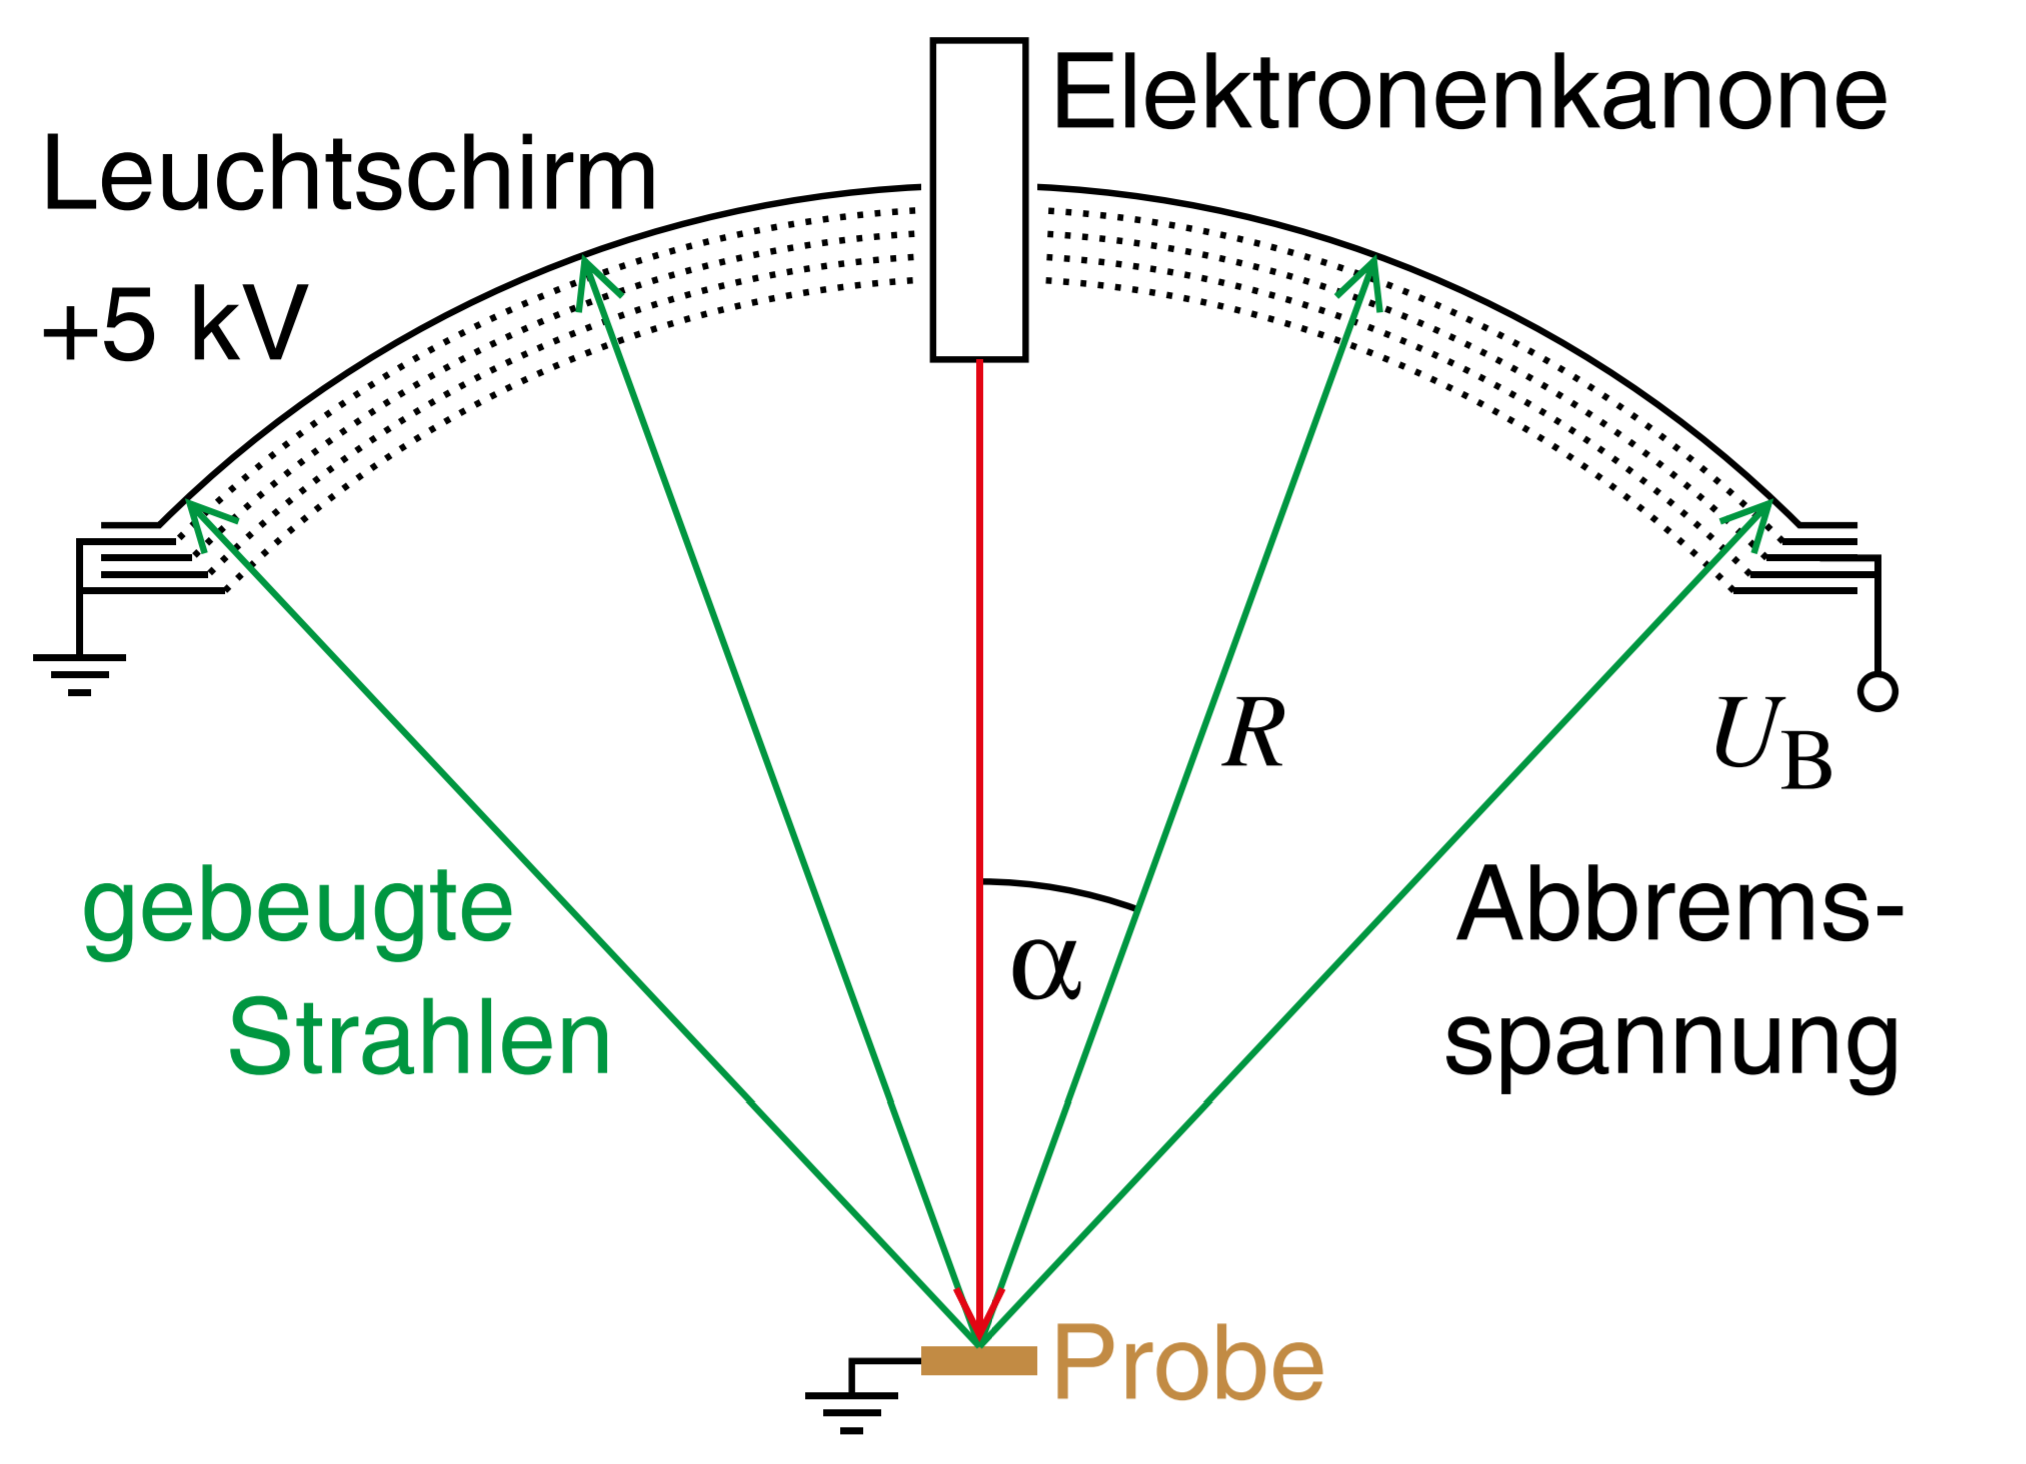
\includegraphics[width=0.5\linewidth]{Plots/LEED_Schema.png}
        \caption{Schematische Darstellung einer LEED-Optik. In grün ist die Bahn der elastisch gestreuten Elektronen zu sehen,
        welche unter dem Winkel $\alpha$ an der Probe gebeugt werden und auf den gekrümmten Leuchtschirm mit Radius $R$ treffen.
        Am Gitter liegt eine Abbremsspannung $U_{\symup{B}}$ an, um inelastisch gestreute Elektronen auszufiltern \cite{fauster}.}
        \label{fig:LEED_Schema}
\end{SCfigure}

Die Beugungsintensität $I$ hängt vom Formfaktor $F$ und vom Gitterfaktor $G$ ab
\begin{equation}
        I=|F|^2\cdot |G|^2.
        \label{eq:LEED}
\end{equation}

Es gilt nur dann $G\neq 0$, wenn die Laue-Bedingung $\symup{\Delta}\vec{k}_{||}=\vec{g}_{hk}$ für den Impulsübertrag in senkrechter Richtung erfüllt ist.
$\vec{g}_{hk}$ bezeichnet hier einen diskreten reziproken Gittervektor.
Es treten also nur bestimmte Beugungsreflexe auf, die durch die Bezeichnung ($hk$) identifiziert werden.
Die Beugungsreflexe geben ein Bild des reziproken Raums der Oberfläche wieder
und sind charakteristisch für die Oberflächenstruktur der Probe.
Ist die Ordnung der Oberfläche zum Beispiel durch Fremdatome gestört, treten weitere Streueffekte auf und
die Reflexe verlieren an Schärfe.

Nach Gleichung \ref{eq:LEED} wirken sich unterschiedliche Strukturen direkt auf die Reflex-Intensität aus, 
weshalb  diese zur Charakterisierung eines Materials verwendet werden kann.
Dafür werden so genannte IV-Kurven genutzt, die die Intensitätsverläufe einzelner Reflexe in Abhängigkeit der Energie 
wiedergeben.
\newpage

\section{MEED}
Die Beugung mittelenergetischer Elektronen (Medium-Energy Electron Diffraction, "MEED") kann in einem Reflektionsaufbau \ref{fig:MEEDS} 
genutzt werden, um die Anzahl der Monolagen während des Wachstums zu bestimmen.

\begin{figure}[H]
        \centering
        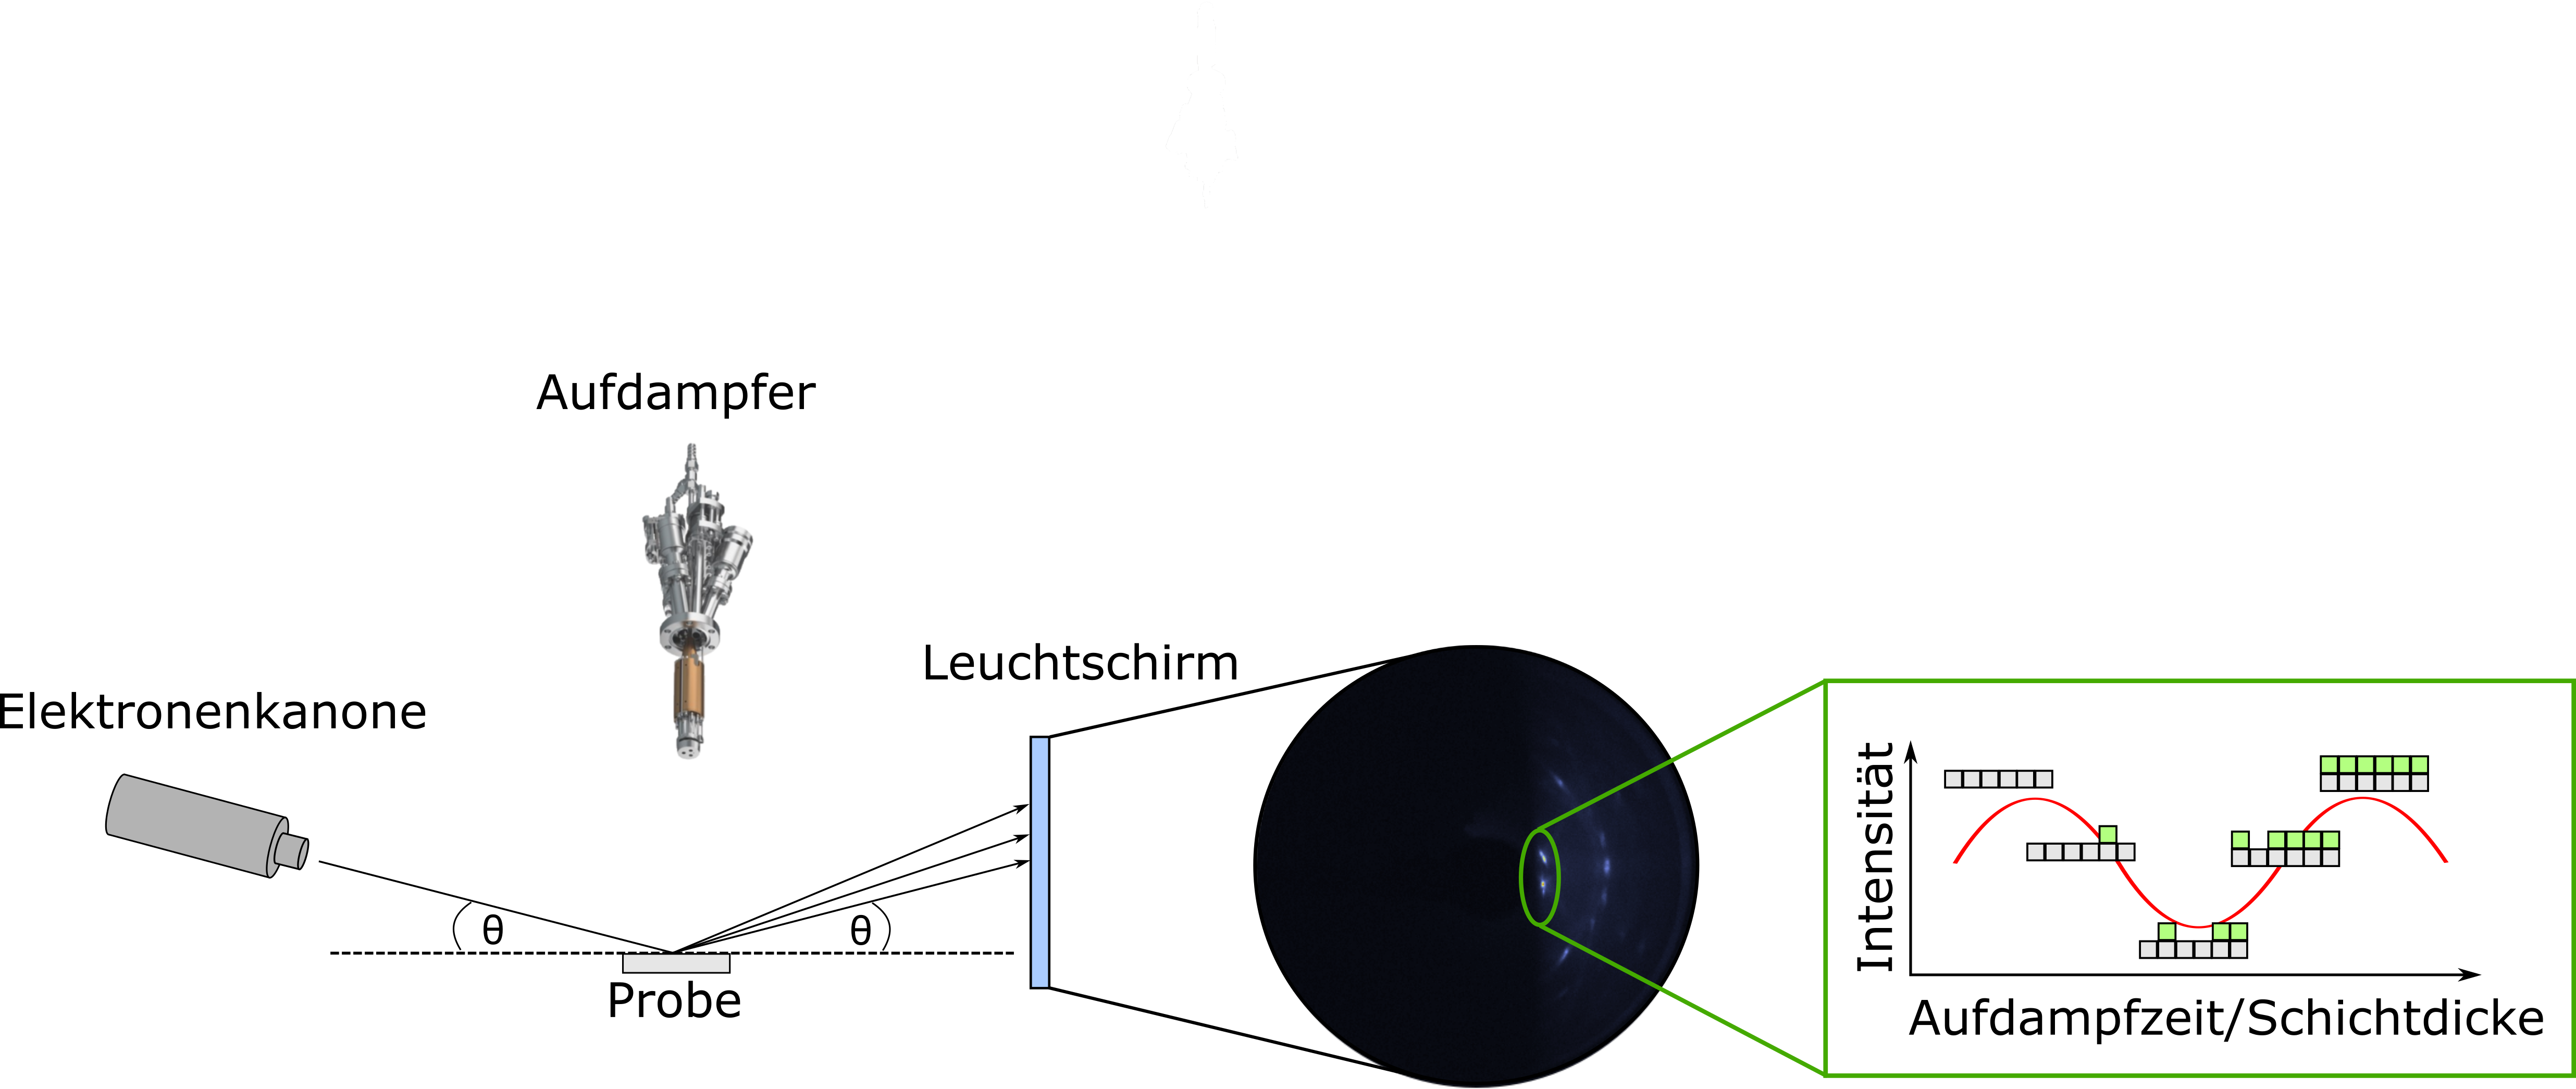
\includegraphics[width=\linewidth]{Plots/MEED_3.pdf}
        \caption{Schematische Darstellung der MEED-Methode im Reflexionsaufbau. Die Elektronenkanone befindet sich gegenüber des
                Leuchtschirms, der Elektronenstrahl kann so in einem flachen Winkel $\Theta$ auf die Probe treffen.
                Dort werden die Elektronen wie bei der LEED-Methode elastisch gestreut und bilden ein Beugungsbild am Leuchtschirm.
                Befindet sich der Aufdampfer \cite{FOCUS} wie abgebildet vor der Probe, kann das Beugungsbild 
                während des Wachstums beobachtet werden. Die Intensität der Beugungsreflexe oszilliert mit der Schichtdicke.
                Mit freundlicher Genehmigung von David Janas.}
        \label{fig:MEEDS}
\end{figure}

Die Intensität der Beugungsreflexe oszilliert dabei in Abhängigkeit der Struktur der Oberfläche.
Die beste Ordnung und demnach die höchste Intensität besteht bei einer abgeschlossenen vollen Monolage.
Bei einem lagenweisen Wachstum kann nun die Bildung einer neuen Lage zunächst durch einen Abfall der Intensität beobachtet werden, 
auf den ein erneuter Anstieg folgt, bis die neue Monolage vollständig ist. Anhand der Anzahl der Intensitätsmaxima lässt sich so die
Anzahl der Monolagen beim Wachstum dünner Schichten bestimmen \cite{neave1983dynamics}. 




\newpage
\section{Augerelektronenspektroskopie}
\label{sec:Auger}
Eine oberflächensensitive Methode zur quantitativen Elementanalyse einer Probe ist die Augerelektronenspektroskopie (Auger Elektron Spectroscopy, "AES").
Mit Hilfe der mittleren freien Weglänge von Elektronen in den entsprechenden Systemen lässt sich aus den Peak-Verhältnissen eines Auger-Spektrums außerdem die Schichtdicke bestimmen.

Wird in einem Atom ein Elektron aus einer inneren Schale z.B. durch Elektronenstrahlung herausgelöst,
wird das entstehende Loch durch ein Elektron einer äußeren Schale aufgefüllt. 
Wenn die dabei frei werdende Energie an ein weiteres Elektron übertragen wird,
kann dieses den Festkörper verlassen und wird Augerelektron genannt.
Dessen Energie ist dabei abhängig von den beteiligten Energieniveaus des Atoms, und somit elementspezifisch.
Wird die Anzahl der detektierten Elektronen in Abhängigkeit ihrer Energie aufgetragen, bilden sich bei den entsprechenden Energien 
charakteristische Peaks, wie beispielhaft in Abbildung \ref{fig:Auger-BSP} gezeigt. Die Intensität wird dabei in differentieller Form dargestellt,
um die Peaks vor dem Untergund inelastisch rückgestreuter Elektronen und Sekundärelektronen hervorzuheben.

\begin{figure}[H]
        \centering
        \includegraphics[width=0.7\linewidth]{Plots/plotAuger2_Layout.pdf}
        \caption{Augerspektrum einer dünnen MgO-Schicht auf Fe(100). Die Elementzugehörigkeiten der gemessenen Peaks sind entsprechend gekennzeichnet.}
        \label{fig:Auger-BSP}
\end{figure}


Um unterschiedliche elementspezifische Faktoren, wie die Wahrscheinlichkeit für einen Augerzerfall,
bei den relativen Peak-Verhältnissen einbeziehen zu können,
werden relative Sensitivitäten $S_{\symup{i}}$ des Elements i definiert, welche empirisch bestimmt werden \cite{davis-1978}.
Die für das zu untersuchende System wichtigen Sensitivitäten von Fe, O und Mg sind in Tabelle \ref{tab:AugerS} aufgetragen.
Die Elementkonzentration $c_{\symup{i}}$ kann so mit der Gleichung 

\begin{equation}
        c_{\symup{i}}=\dfrac{{I_{\symup{i}}}/{S_{\symup{i}}}}{\sum_{\symup{j}}{I_{\symup{j}}}/{S_{\symup{j}}}}
        \label{eq:AugerK}
\end{equation}

bestimmt werden, wobei $I_{\symup{i}}$ die Peak-Intensität bezeichnet. Die Summe läuft über alle vorhandenen Elemente j \cite{fauster}.

\begin{table}[H]
        \centering
        \begin{tabular}{S | S}
          \toprule
          {$\symup{Element}$} & {$S_{\symup{i}}$}\\
          \midrule
          $\symup{Fe \:(651\,eV)}$ & {$0,2$}\\
          $\symup{O \:(503\,eV)}$ & {$0,5$} \\
          $\symup{Mg \:(1174\,eV)}$ & {$0,1$}\\
          \bottomrule
        \end{tabular}
        \caption{Relative Sensitivitäten $S_{\symup{i}}$ der untersuchten Elemente Fe, O und Mg \cite{davis-1978}.}
        \label{tab:AugerS}
\end{table}
Um die Schichtdicke aus Augerspektren zu bestimmen, ist es wichtig, die mittleren freien Weglängen $\lambda$ von Elektronen bei den Energien zu kennen, 
bei denen die charakteristischen Peaks auftreten. In der Literatur lassen sich verschiedene mittlere freie Weglängen finden,
wovon einige in Tabelle \ref{tab:AugerM} aufgeführt sind.

\begin{table}
        \centering
        \begin{tabular}{c| c c c c}
          \toprule
          Energie & Gries \cite{gries1996universal} & Tanuma et al. \cite{tanuma1994calculations}& Akermann et al. \cite{akkerman1996inelastic}& Seah et al. \cite{seah1979quantitative}\\
          \midrule
          {$651\,\si{\eV}$} & {$14,62\,\si{\angstrom}$} & {$16,35\,\si{\angstrom}$} & {$15,48\,\si{\angstrom}$} & {$18,9\,\si{\angstrom}$}\\
          {$503\,\si{\eV}$} & {$12,70\,\si{\angstrom}$} & {$13,65\,\si{\angstrom}$} & {$12,69\,\si{\angstrom}$} & {$16,7\,\si{\angstrom}$}\\
          {$1174\,\si{\eV}$} & {$22,55\,\si{\angstrom}$}& {$25,34\,\si{\angstrom}$}& {$24,72\,\si{\angstrom}$}& {$23,5\,\si{\angstrom}$}\\
          \bottomrule
        \end{tabular}
        \caption{Mittlere freie Weglängen bei den relevanten Energien in MgO \cite{Wachstum}.}
        \label{tab:AugerM}
      \end{table}


\begin{equation}
        \dfrac{I_{\symup{A}}}{I_{\symup{S}}}=\dfrac{S_{\symup{A}}\cdot \left( 1-\symup{exp}\left( -\dfrac{d}{0,74\cdot \lambda_{\symup{A}}} \right) \right) }  {S_{\symup{S}}\cdot \symup{exp} \left( -\dfrac{d}{0,74 \cdot\lambda_{\symup{S}}} \right) }
        \label{eq:Auger-V}
\end{equation} 

Gleichung \ref{eq:Auger-V} stellt einen Zusammenhang zwischen dem Augerpeak-Verhältnis des Adsorbats $I_{\symup{A}}$ zum Substrat $I_{\symup{S}}$ und der Schichtdicke $d$
des Absorbats her \cite{Wachstum}. 
\newpage


\section{Experimentelles Setup}

\begin{SCfigure}
        \centering
        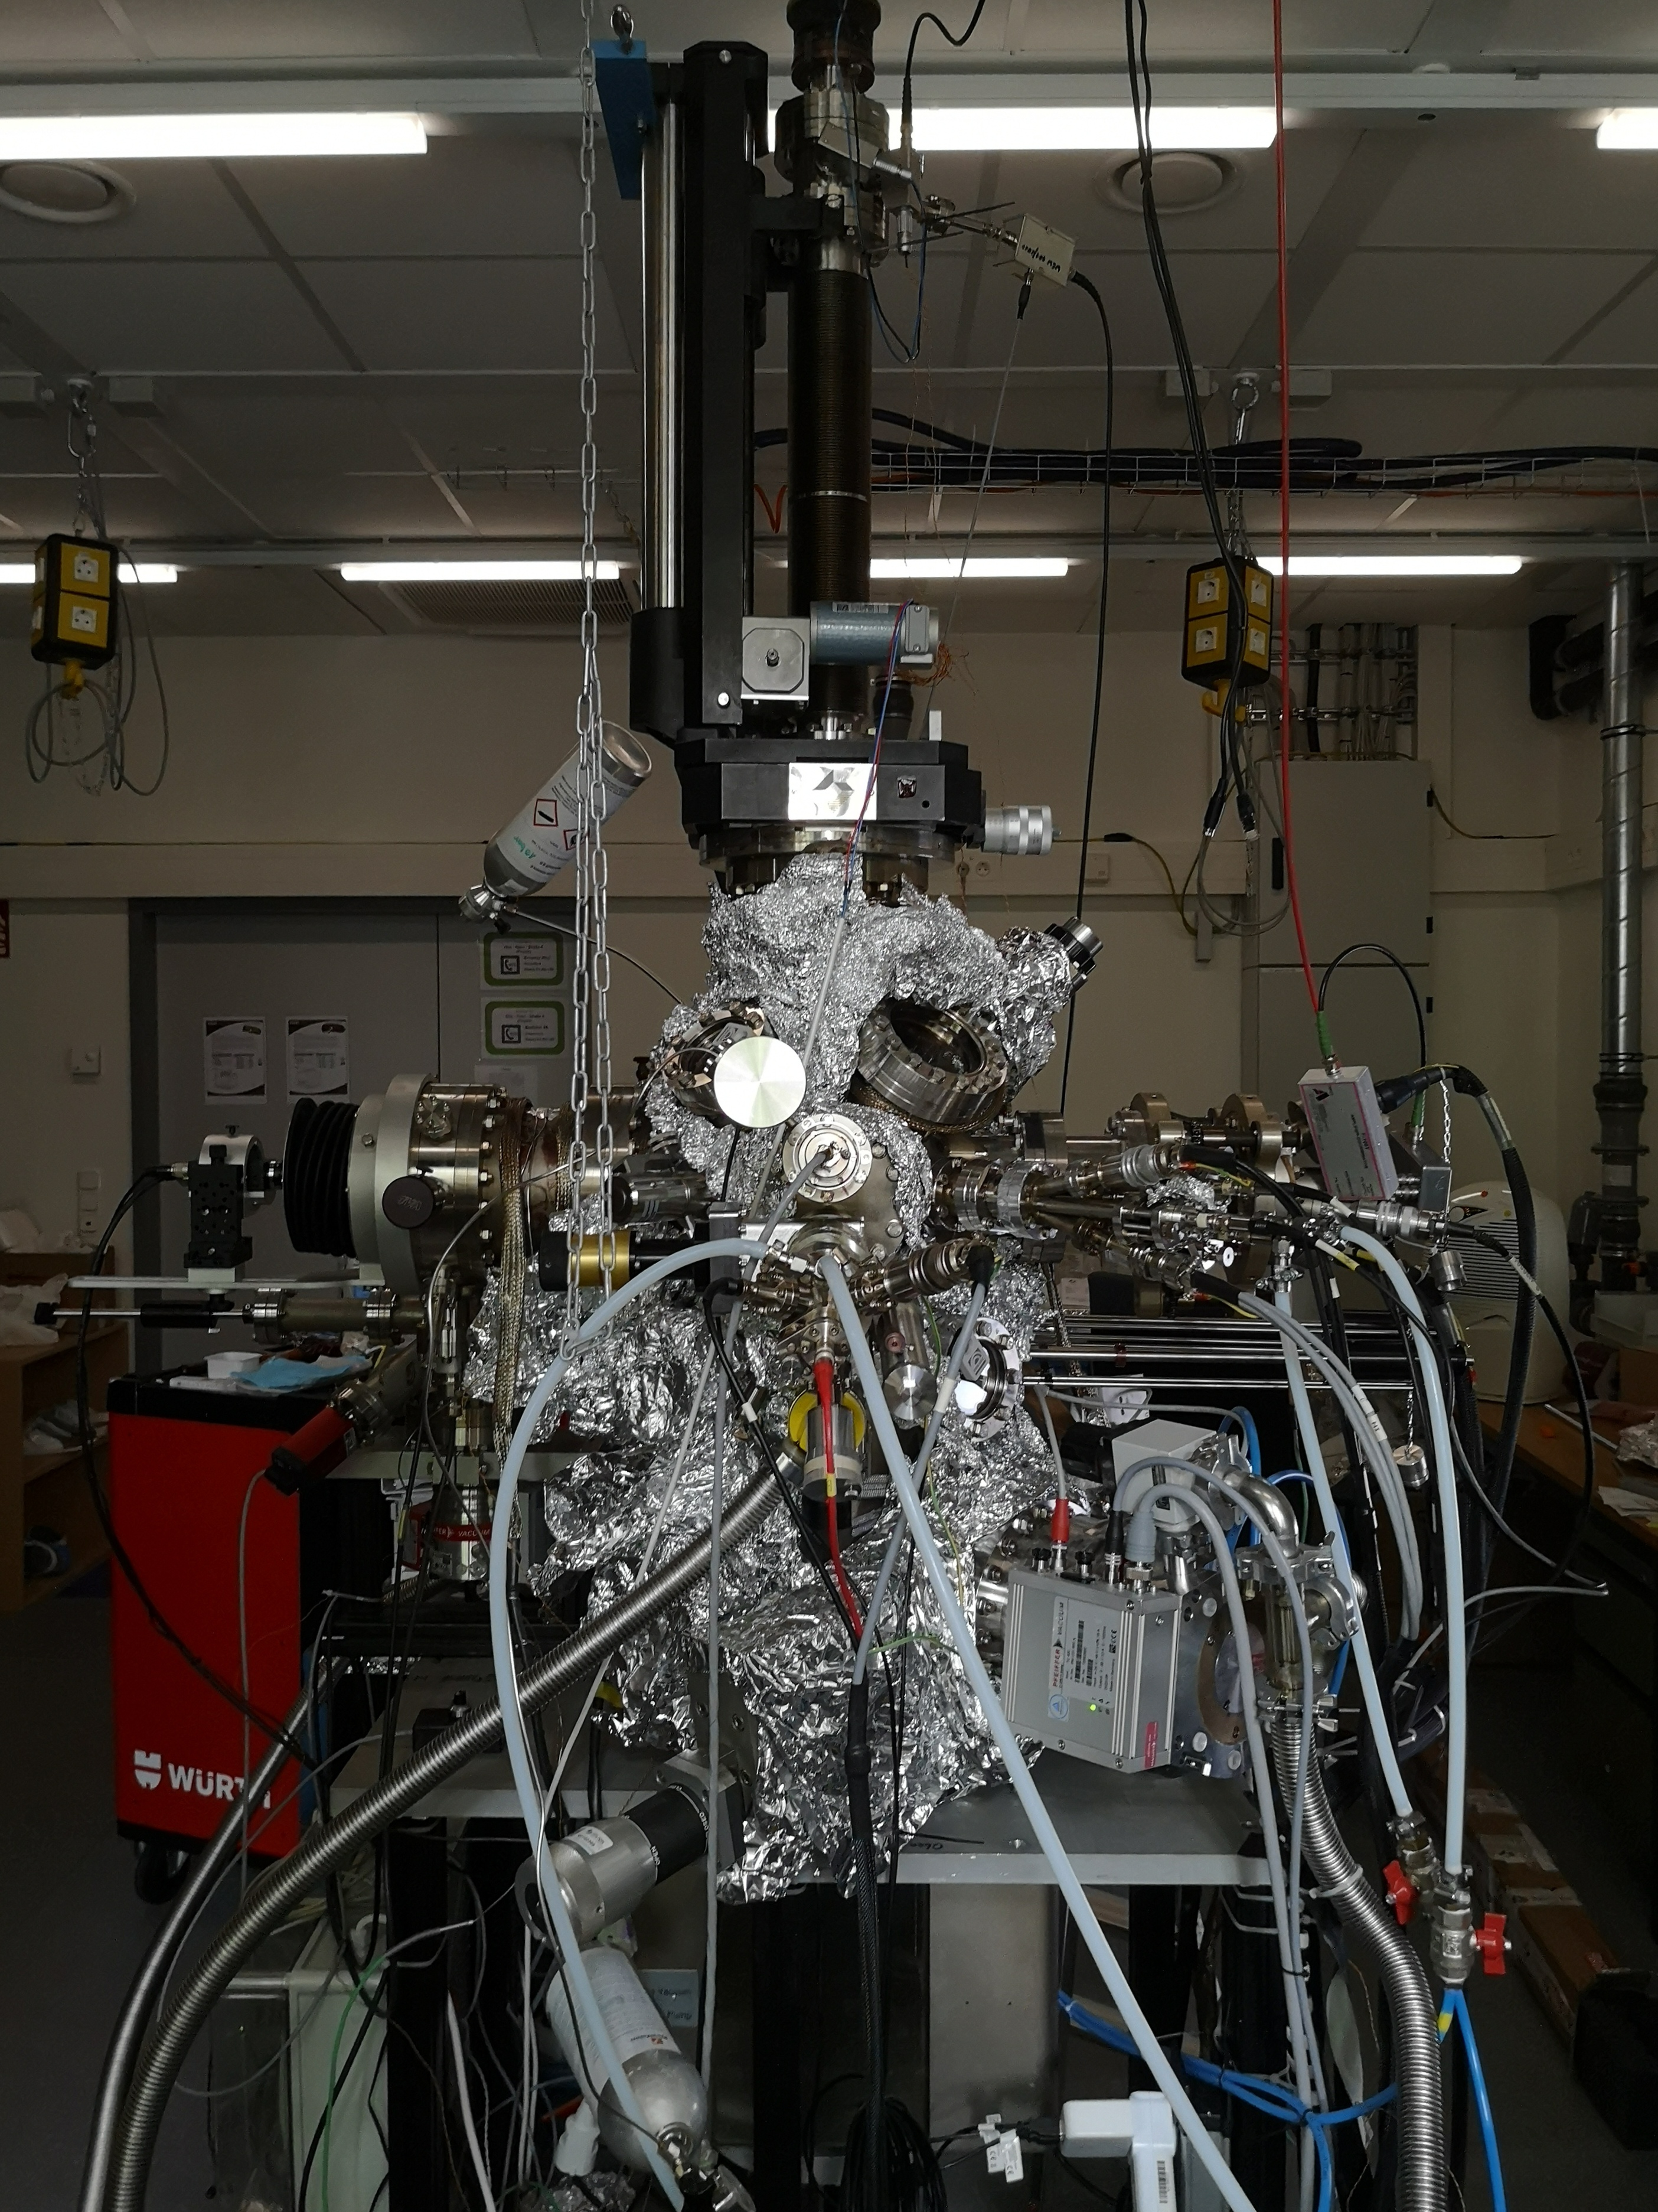
\includegraphics[width=0.6\linewidth]{Plots/BILD_PREP.pdf}
        \caption{Gezeigt ist die verwendete Präperationskammer. Beschriftet sind die Komponenten des Reflektions-MEED Aufbaus.}
        \label{fig:BILD_PREP}
\end{SCfigure}

Das Wachstum wurde in einer Ultra-Hoch Vakuum (UHV) Kammer durchgeführt, die auf das Wachstum und die Analyse dünner Schichtsysteme ausgelegt ist.
Der Basisdruck in der Kammer liegt in der Größenordnung von $p=6\cdot 10^{-11}\,\si{\milli\bar}$.
Zur ständigen Druckmessung wird dabei ein Ionisations-Vakuummeter verwendet.
In die Kammer können über Leckventile $\symup{Ar}^+$-Ionen sowie $\symup{O_2}$-Moleküle 
eingelassen werden. 

Die $\symup{Ar}^+$-Ionen werden dabei zum Reinigen der Probe mittels ioneninduzierter Zerstäubung (sputtering) verwendet.
Sie können durch eine angelegte Spannung unter einem Winkel auf die Probe beschleunigt werden und tragen durch Stöße Oberflächenatome ab.
Anschließendes Heizen der Probe mit einem Heizwiderstand sorgt für die Desorption weiterer Verunreinigungen sowie eine Neuordnung der 
Oberfläche durch zusätzliche thermische Energie.
 Die Temperatur wird mit einem Thermoelement gemessen, welches sich leicht entfernt von der Probe befindet, weshalb 
eine kleine Differenz zur tatsächlichen Temperatur der Probe vorliegt.

Die Probe ist in der Kammer durch einen Manipulator frei translatierbar und zudem um $360\,\si{\degree}$ um die z-Achse rotierbar.
Am Manipulator ist außerdem eine QCM befestigt, die in der Höhe und  Tiefe versetzt zur Probenhalterung angebracht ist.

Das Magnesium wird aus Pellets mit $99,99\,\si{\percent}$ Reinheit aus einem Molybdän-Tiegel aufgedampft.
Der Aufdampfer steht dabei in einem Winkel von $90\,\si{\degree}$ zum LEED-Schirm und zur Elektronenkanone des AES, was MEED-Messungen während des Aufdampfens ermöglicht.
Für unterschiedliche Winkel zwischen Probe und LEED-Schirm stellen sich verschiedene Beugungsordnungen ein, welche in Abbildung \ref{fig:MEED-Bilder} zu sehen sind.



\begin{figure}[H]
    \centering
    \subfloat[][]{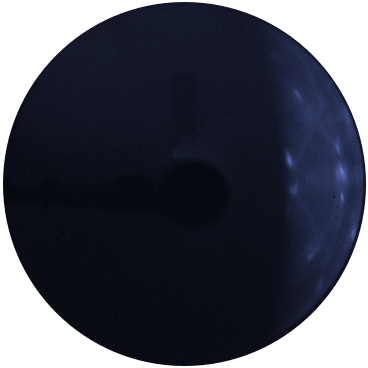
\includegraphics[width=0.28\linewidth]{Plots/MEED_103_degree.png}}%
    \qquad
    \subfloat[][]{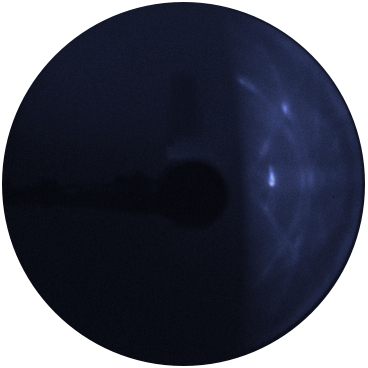
\includegraphics[width=0.28\linewidth]{Plots/MEED_109_degree.png}}%
    \qquad
    \subfloat[][]{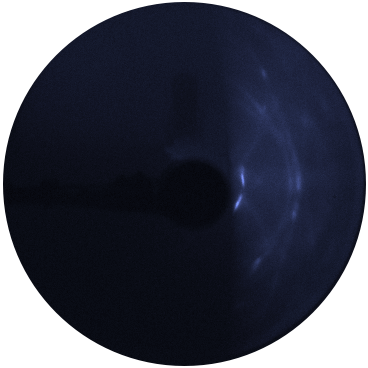
\includegraphics[width=0.28\linewidth]{Plots/MEED_113_degree.png}}%
    \caption{Bilder des LEED-Schirms mit MEED-Einstellungen für verschiedene Winkel zwischen Probe und Schirm. 
            (a) zeigt einen Winkel von $\Theta=13\,\si{\degree}$, (b) einen Winkel von $\Theta=7\,\si{\degree}$ und (c) einen Winkel von $\Theta=3\,\si{\degree}$ zwischen Probe und Schirm.}%
    \label{fig:MEED-Bilder}
  \end{figure}



%\chapter{Preparationskammer}

Das Wachstum wurde in einer Ultra-Hoch Vakuum (UHV) Kammer durchgeführt, die auf das Wachstum und die Analyse dünner Schichtsysteme ausgelegt ist.
Der Basisdruck in der Kammer liegt in der Größenordnung von $p=1\cdot 10^{-10}\,\si{\milli\bar}$.
Zur ständigen Druckmessung wird dabei ein Ionisations-Vakuummeter (ion gauge) verwendet.
In die Kammer können über leak Ventile $\symup{Ar}^+$-Ionen sowie $\symup{O_2}$-Moleküle 
eingelassen werden. 

Die $\symup{Ar}^+$-Ionen werden dabei zum Reinigen der Probe bei der Ioneninduzierten Zerstäubung (sputtering) verwendet.
Diese können durch eine angelegte Spannung unter einem Winkel auf die Probe beschleunigt werden und tragen durch Stöße Oberflächenatome ab.
Durch anschlißendes Heizen der Probe desorbieren weitere Verunreinigungen und durch die zusätzliche thermische Energie ordnet sich die 
Oberfläche neu.

Die Probe ist in der Kammer durch einen Manipulator frei translatierbar und außerdem um $360\,\si{\degree}$ um die z-Achse rotierbar.
Am Manipulator ist außerdem eine QCM befestigt, die in der Höhe und  Tiefe versetzt zur Probenhalterung angebracht ist.

Der MG-Aufdampfer steht im $90\,\si{\degree}$ Winkel zum LEED Schrim und zur Elektronenquelle des AES, was MEED Messungen während des Aufdampfens ermöglicht.
Für unterschiedliche Winkel zwischen Probe und LEED Schirm stellen sich verschiedene Beugungsordnungen ein, welche in Abbildung \ref{fig:MEED-Bilder} zu sehen sind.



\begin{figure}[H]
    \centering
    \subfloat[][]{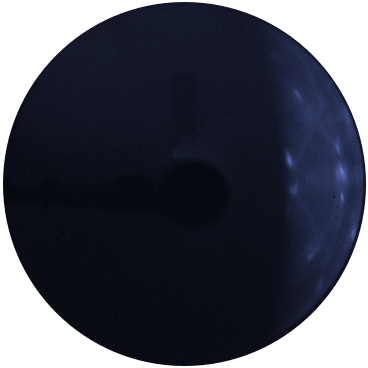
\includegraphics[width=0.28\linewidth]{Plots/MEED_103_degree.png}}%
    \qquad
    \subfloat[][]{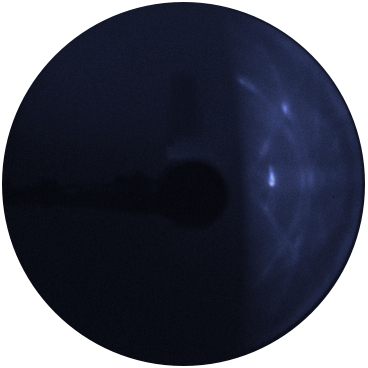
\includegraphics[width=0.28\linewidth]{Plots/MEED_109_degree.png}}%
    \qquad
    \subfloat[][]{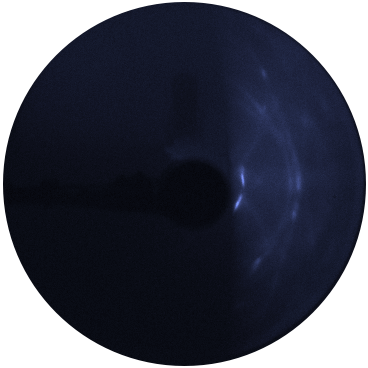
\includegraphics[width=0.28\linewidth]{Plots/MEED_113_degree.png}}%
    \caption{Bilder des LEED Schirms mit MEED Einstellungen für verschiedene Winkel zwischen Probe und Schirm. 
            (a) zeigt einen Winkel von $13\,\si{\degree}$, (b) einen Winkel von $7\,\si{\degree}$ und (c) einen Winkel von $3\,\si{\degree}$ zwischen Probe und Schirm.}%
    \label{fig:MEED-Bilder}
  \end{figure}


\chapter{Ergebnisse}
Die verwendete Fe(100)-Oberfläche wurde gefertigt, 
indem ein dünner Eisenfilm (ca. $200\,\si{\nano\meter}$\,-\,$400\,\si{\nano\meter}$) auf einen MgO(100)-Kristall aufgedampft wurde.

Um eine saubere Fe(100)-Oberfläche zu erhalten,
wurde die Probe zunächst durch mehrere Sputter- und Heizdurchgänge
gereinigt. Bei je einem Durchgang wurde bei einer Spannung von $U=1\,\si{\kilo\volt}$ und 
einem Argondruck von $p=1\cdot 10^{-5}\,\si{\milli\bar}$ für 
$15\,\si{\minute}$ gesputtert
und für $5\,\si{\minute}$ bei einer Temperatur von $T=600\,\si{\celsius}$ geheizt. Mittels Auger-Spektren und LEED-Bildern 
wurde die Reinheit und Ordnung der Oberfläche überprüft. 
Solch ein Auger-Spektrum und ein LEED-Bild von der sauberen Fe(100) Oberfläche sind in den Abbildungen \ref{fig:Auger1} 
(oben) und  \ref{fig:LEED} (a) zu sehen.



Auf der gereinigten Probe wurde nun das MgO-Wachstum einzelner Monolagen untersucht.
Die Mg-Aufdampfrate wurde mittels der QCM bestimmt 
und damit anschließend bei passendem Sauerstoffdruck nach Zusammenhang \ref{eq:V1} 
eine MEED-Messung des Wachstums von MgO bei einer Probentemperatur von $T=170\,\si{\celsius}$
für $22\,\si{\minute}$ auf dem sauberen Eisen durchgeführt. 
Eine höhere Temperatur erleichtert zwar das lagenweise Wachstum, doch 
nach Tekiel et al. sinkt die kristalline Ordnung bei Temperaturen über $T=160\,\si{\celsius}$ \cite{tekiel2013reactive}. 
Wegen der Distanz des Thermoelements zur Probe wurde hier eine etwas höhere Temperatur von $T=170\,\si{\celsius}$ gewählt.

Um den Prozess mit Auger-Spektren, LEED-Bildern und IV-Kurven zu untersuchen, wurde das gleiche Wachstum noch einmal 
sukzessive durchgeführt. Dabei wurde die Probe je einmal vollständig mit diesen Methoden vermessen und anschließend 
bei den gleichen Einstellungen wie oben Magnesium nacheinander für je $t=116\,\si{\second}$, $t=250\,\si{\second}$, $t=597\,\si{\second}$ 
und $t=251\,\si{\second}$ in Sauerstoffatmosphäre aufgedampft.

Für den Vergleich mit dem Wachstum von MgO auf passivertem Eisen wurde auch dieses System vermessen.
Zur Passiverung wurde die saubere Eisenprobe zunächst für $5\,\si{\minute}$ bei einer Temperatur von $T=550\,\si{\celsius}$ 
und einer Sauerstoffatmosphäre mit 
$p=1,3\cdot 10^{-7}\,\si{\milli\bar}$ ausgesetzt, was $30\,\symup{L}$ entspricht. 
Nach \cite{picone2016controlling} bildet sich auf diese Weise eine Fe(100)-p(1\,x\,1)O Struktur.
\newpage
\section{Schichtdicken-Charakterisierung mittels MEED und AES}

In Abbildung \ref{fig:QCM1} ist die aufgedampfte Mg-Schichtdicke in Abhängigkeit der Zeit aufgetragen.
Im Bereich von $t=400\,\si{\second}$ bis $t=600\,\si{\second}$ wurde der Aufdampfer mit einem Flux von $130\,\si{\nano\ampere}$ betrieben, 
welcher als finale Einstellung auch beim MgO-Wachstum verwendet wurde.

\begin{SCfigure}
  \centering
  \includegraphics[scale=1, width=0.5\linewidth]{Plots/QCM_Layout.pdf}
  \caption{Aufgedampfte Mg-Schichtdicke auf der QCM vor und nach dem Öffnen des Shutters.
          Aus der Änderung der Schichtdicke mit der Zeit ergibt sich eine Aufdampfrate von $r=0,34\,\si{\angstrom\per\minute}$.}
  \label{fig:QCM1}
\end{SCfigure}

Aus der dadurch resultierenden Aufdampfrate von $r=0,34\,\si{\angstrom\per\minute}$ und dem verwendeten 
Sauerstoffdruck $p=3\cdot 10^{-8}\,\si{\milli\bar}$ ergibt sich ein Verhältnis von

\begin{equation*}
  \frac{r}{p}=0,11\cdot 10^8 \,\si{\angstrom\per\milli\bar\per\minute},
\end{equation*}

welches im Bereich $r/p=(0,15\pm 0,05)\cdot 10^8 \,\si{\angstrom\per\milli\bar\per\minute}$ (siehe Abschnitt \ref{sec:Wachstum}) liegt.

\begin{figure}[H]
  \centering
  \includegraphics[scale=1, width=0.7\linewidth]{Plots/MEED-Original-2_Layout.pdf}
  \caption{MEED-Spektrum des MgO-Wachstums auf Fe(100). Aufgedampft wurde mit einer Rate von $r=0,34\,\si{\angstrom\per\minute}$ 
          bei einem Sauerstoffdruck von $p=3\cdot 10^{-8}\,\si{\milli\bar}$.}
  \label{fig:MEED1}
\end{figure}

Der in Abbildung \ref{fig:MEED1} gezeigte MEED-Verlauf zeigt die Maxima der ersten zwei vollen Monolagen nach $106\,\si{\second}$ und weiteren $281\,\si{\second}$.
Aufgrund des starken Untergrunds lässt sich das Maxima der dritten Monolage nicht so eindeutig und  das der vierten Monolage gar nicht zuordnen, 
doch der relative Verlauf und die Ergebnisse der späteren Auswertung der Augerpeak Verhältnisse lässt darauf schließen, dass sich
die dritte Monolage nach weiteren $352\,\si{\second}$ und die vierte Monolage sich nach weiteren $345\,\si{\second}$ bildet. 

Auffällig ist hier, dass die Wachstumszeit für eine volle Monolage nicht konstant ist, sondern sich einem Grenzwert von ca. $350\,\si{\second}$ annähert.

Aus der Mg-Aufdampfrate der QCM lässt sich eine Vorhersage für die MgO-Wachstumsrate erstellen. Dazu wird angenommen, dass 
bei einem MgO-Kristall die Hälfte der Gitterplätze mit Sauerstoffatomen belegt ist, wodurch sich die MgO-Wachstumsrate gegenüber der Mg-Aufdampfrate
verdoppeln würde. Jedoch ist auch die Dichte von MgO um den Faktor $\rho_{\symup{MgO}}/\rho_{\symup{Mg}}=2,06$ größer als die von Mg, weshalb
sich die Wachstumsrate durch die dichtere Anordnung verringert. Insgesamt ergibt sich so $r_{\symup{Wachstum,\, QCM}}=0,97\cdot r=0,33\,\si{\angstrom\per\minute}$.
Zwischen der so ermittelten und der gemessenen Wachstumsrate $r_{\symup{Wachstum,\, MEED}}=0,36\,\si{\angstrom\per\minute}$ von MgO (angenommen wurde eine Schichtdicke von 2,105$\si{\angstrom}$) 
besteht also ein Faktor 

\begin{equation*}
  \frac{r_{\symup{Wachstum,\, MEED}}}{r_{\symup{Wachstum,\, QCM}}}=1,09.
\end{equation*}

Um die variierende Wachstumszeit genauer zu untersuchen, wird eine 
weitere MEED-Messung des Wachstums von MgO auf Fe(100) und Fe(100)-p(1\,x\,1)O 
zum Vergleich der beiden Systeme betrachtet.
Die Aufdampfrate für diese Messung wurde 
mittels der QCM zu $r=0,45\,\si{\angstrom\per\minute}$ bestimmt (Abbildung \ref{fig:QCM2}).

\begin{SCfigure}
  \centering
  \includegraphics[scale=1, width=0.5\linewidth]{Plots/QCM_2021_07_21_Layout.pdf}
  \caption{Aufgedampfte Mg-Schichtdicke auf der QCM vor und nach dem Öffnen des Shutters.
  Aus der Änderung der Schichtdicke mit der Zeit ergibt sich eine Aufdampfrate von $r=0,45\,\si{\angstrom\per\minute}$.}
  \label{fig:QCM2}
\end{SCfigure}



\begin{figure}[H]
  \centering
  \includegraphics[scale=1, width=0.7\linewidth]{Plots/MEED_2021_07_21_FeO_u_Fe_Layout.pdf}
  \caption{MEED-Messungen des MgO-Wachstums auf Fe(100) (orange) und Fe(100)-p(1\,x\,1)O (blau). Die Messungen wurden um einen linear verlaufenden Untergrund korrigiert.
          Aufgedampft wurde mit einer Rate von $r=0,45\,\si{\angstrom\per\minute}$ 
          bei einem Sauerstoffdruck von $p=4\cdot 10^{-8}\,\si{\milli\bar}$.}
  \label{fig:MEED2}
\end{figure}

Die Oszillationen im MEED-Verlauf \ref{fig:MEED2} sind bei dieser Messung deutlich zu erkennen und können durchgängig 
den vollen Monolagen des Wachstums zugeordnet werden. Beim passivierten Eisen ist die Wachstumszeit nahezu konstant bei $258\,\si{\second}$ für eine volle Monolage.
Auch hier stellt sich der Faktor von

%Die Oszillationen im MEED Verlauf \ref{fig:MEED2} sind bei dieser Messung deutlich zu erkennen und können durchgängig eindeutig 
%den vollen Monolagen des Wachstums zugeordnet werden. Hierbei ist die Wachstumszeit nahezu konstant bei $258\,\si{\second}$ für eine volle Monolage.
%Auch hier stellt sich der Faktor von
%
\begin{equation*}
  \frac{r_{\symup{Wachstum,\, MEED}}}{r_{\symup{Wachstum,\, QCM}}}=1,09
\end{equation*} 

zwischen der Wachstumsrate $r_{\symup{Wachstum,\, QCM}}=0,97\cdot r=0,44\,\si{\angstrom\per\minute}$ und 
der bestimmten Wachstumsrate $r_{\symup{Wachstum,\, MEED}}=0,48\,\si{\angstrom\per\minute}$ ein.

Es ist wieder zu beobachten, dass die ersten zwei ML auf dem reinen Eisen schneller wachsen als die Nachfolgenden.
Später stellt sich die gleiche Wachstumszeit für eine ML ein wie beim passivierten Eisen.
Dies lässt sich auf die hohe Reaktivität der reinen Eisenoberfläche zurückführen.
Während also bei dem MgO Wachstum auf reinem Eisen der Sauerstoff besonders schnell auf der Eisenoberfläche adsorbiert, 
so ist das passivierte Eisen schon mit Sauerstoff gesättigt und das Wachstum von Beginn an gleichbleibend schnell.

Die Schichtdickenbestimmung mit AES-Spektren wurde bei MgO-Wachstum auf sauberem Fe(100) durchgeführt.
Die aufgenommenen Spektren des sukzessiven Wachstums sind in Abbildung \ref{fig:Auger1} dargestellt.

\begin{SCfigure}
  \centering
  \includegraphics[scale=1, width=0.7\linewidth]{Plots/Auger_Vergleich_Layout.pdf}
  \caption{Auger-Spektren im Energiebereich $E=200-1250\, \si{\eV}$ nach unterschiedlicher Aufdampfdauer. 
          Die Bestimmung der Anzahl der ML erfolgt später durch \ref{fig:Auger-Verhältnisse2}. Durch einen Savitzky-Golay Filter 2.\nobreakspace Ordnung mit 9 Punkten wurden die
          Auger-Spektren geglättet.}
  \label{fig:Auger1}
\end{SCfigure}



\begin{figure}[H]
  \centering
  \includegraphics[width=\linewidth]{Plots/Auger-Verhältnisse-Schichtdicke_2_Layout.pdf}
  \caption{Augerpeak-Verhältnisse in Abhängigkeit der Schichtdicke errechnet mit Gleichung \ref{eq:Auger-V}, für die verschiedenen
           mittleren freien Weglängen aus \ref{tab:AugerS}. Dabei geben die blauen Kurven das O/Fe Verhältnis und die schwarzen Kurven das Mg/Fe Verhältnis an.
           Die Kreuze kennzeichnen die gemessenen Verhältnisse nach ausgewählten Aufdampfdauern.}
  \label{fig:Auger-Verhältnisse1}
\end{figure}

Die Auswertung der Verhältnisse der Peaks für verschiedene mittlere freie Weglängen nach Gleichung \ref{eq:Auger-V} ist in Abbildung \ref{fig:Auger-Verhältnisse1} zu sehen.
Dabei stimmen die Schichtdicken der Mg/Fe und der O/Fe-Verhältnisse mit den mittleren freien Weglängen von Seah et al. \cite{seah1979quantitative} am besten überein.
Diese sind noch einmal in Abbildung \ref{fig:Auger-Verhältnisse2} dargestellt.

\begin{SCfigure}
  \centering
  \includegraphics[width=0.7\linewidth]{Plots/Auger-Verhältnisse-Schichtdicke_Layout.pdf}
  \caption{Augerpeak-Verhältnisse in Abhängigkeit der Schichtdicke errechnet mit Gleichung \ref{eq:Auger-V} und den mittleren freien Weglängen von Seah et al. \cite{seah1979quantitative}, je einmal für das Mg/Fe- und das O/Fe-Verhältnis.
          Die Kreuze kennzeichnen die gemessenen Verhältnisse nach ausgewählten Aufdampfdauern.}
  \label{fig:Auger-Verhältnisse2}
\end{SCfigure}


Auf diese Weise lassen sich den Wachstumszeiten jeweils präzise MgO-Schichtdicken zuordnen.
Da es sich um unterschiedliche Wachstumsdurchläufe handelt,
lassen sich die Ergebnisse nur bedingt auf die MEED-Messung \ref{fig:MEED1} übertragen, 
weichen jedoch auch dort nur um maximal $0,5$\,ML von der bestimmten Schichtdicke ab.


\section{Elementanalyse mittels AES}


Aus den aufgenommenen Auger-Spektren \ref{fig:Auger1} lässt sich durch Gleichung \ref{eq:AugerK} die Konzentration der Elemente an der Oberfläche bestimmen,
siehe Tabelle \ref{tab:AugerT}.


\begin{table}
  \centering
  \begin{tabular}{S| S S S S S}
    \toprule
    {$\symup{Element}$} & {$0\,\symup{ML}$} & {$1\,\symup{ML}$} & {$1,6\,\symup{ML}$} & {$3,5\,\symup{ML}$} & {$4,3\,\symup{ML}$}\\
    \midrule
    $\symup{Fe}$ & {$100\,\si{\percent}$} & {$77\,\si{\percent}$} & {$66\,\si{\percent}$} & {$44\,\si{\percent}$} & {$37\,\si{\percent}$}\\
    $\symup{O}$ & {$0\,\si{\percent}$} & {$11\,\si{\percent}$} & {$20\,\si{\percent}$} & {$32\,\si{\percent}$} & {$36\,\si{\percent}$}\\
    $\symup{Mg}$ & {$0\,\si{\percent}$}& {$12\,\si{\percent}$}& {$14\,\si{\percent}$}& {$24\,\si{\percent}$}& {$27\,\si{\percent}$}\\
    \bottomrule
  \end{tabular}
  \caption{Konzentration der vorhandenen Elemente an der Oberfläche nach sukzessivem Wachstum von MgO auf Fe(100).}
  \label{tab:AugerT}
\end{table}

Während zu Beginn die Konzentration des Magnesiums noch gleich der von Sauerstoff ist, stellt sich nach dem zweiten Wachstum ein 
Sauerstoffüberschuss ein. Es scheint also sinnvoll, den Sauerstoffdruck nach der ersten Monolage zu senken, was den Ergebnissen aus \cite{tekiel2013reactive} widerspricht.
Tekiel et al. fanden ein besseres Mg/O-Verhältnis bei niedrigeren Sauerstoffdrücken zu Beginn des Wachstums während der 
ersten Monolage, mit darauf folgenden höheren Sauerstoffdrücken.

Es ist jedoch wichtig anzumerken, dass der Mg-Peak durch die geringe Sensitivität $S=0,1$ bei sehr geringer Konzentration an
der Oberfläche nur schwer vom Untergundrauschen der Augerspektren zu unterscheiden ist. 

\begin{SCfigure}
  \centering
  \includegraphics[scale=1, width=0.69\linewidth]{Plots/Auger_Vergleich__FeO_Layout.pdf}
  \caption{Auger-Spektren im Energiebereich $E=200-1200\, \si{\eV}$ bei unterschiedlichen Schichtdicken von MgO auf Fe-p(1\,x\,1)O. 
          Durch einen Savitzky-Golay Filter 2. Ordnung mit 9 Punkten wurden die
          Auger-Spektren geglättet.}
  \label{fig:Auger2}
\end{SCfigure}



\begin{table}[H]
  \centering
  \begin{tabular}{S| S S S}
    \toprule
    {$\symup{Element}$} & {$0\,\symup{ML}$} & {$1,1\,\symup{ML}$} & {$2,5\,\symup{ML}$}\\
    \midrule
    $\symup{Fe}$ & {$89\,\si{\percent}$} & {$71\,\si{\percent}$} & {$61\,\si{\percent}$}\\
    $\symup{O}$ & {$11\,\si{\percent}$} & {$19\,\si{\percent}$} & {$21\,\si{\percent}$}\\
    $\symup{Mg}$ & {$0\,\si{\percent}$}& {$10\,\si{\percent}$}& {$18\,\si{\percent}$}\\
    \bottomrule
  \end{tabular}
  \caption{Konzentration der vorhandenen Elemente an der Oberfläche nach sukzessivem Wachstum von MgO auf Fe(100)-p(1\,x\,1)O.}
  \label{tab:AugerT2}
\end{table}

Für MgO auf dem passivierten Eisen sind die Auger-Spektren in Abbildung \ref{fig:Auger2} dargestellt und die errechneten Konzentrationen 
in Tabelle \ref{tab:AugerT2} aufgeführt. Während die Mg-Konzentration vergleichbar ist mit der des Wachstum auf reinem Fe(100),
bleibt die Sauerstoffkonzentration beim passivierten Eisen auch nach dem Wachstum weniger Monolagen erhöht. 
Dies zeigt widerum, dass die reine Eisenprobe nicht
sofort passiviert wird, wenn für das Wachstum eine Sauerstoffatmopshäre in der Größenordnung $p=3\cdot 10^{-8}\,\si{\milli\bar}$ eingestellt wird. 
Weiterführend dazu fanden Cattoni et al. \cite{PhysRevB.80.104437} mittels Röntgenphotoelektronenspektroskopie-Messungen heraus, dass keine Fe-O Interaktionen an der Fe(100)/MgO-Grenzfläche 
stattfinden. Die physikalischen Eigenschaften der reinen Eisenoberfläche bleiben im Falle eines 
Fe(100)/MgO-Systems im Vergleich zu einem Fe(100)-p(1\,x\,1)O/MgO-System also erhalten. Zudem wurde bei diesen Schichtsystemen 
eine erhöhte Austauschaufspaltung für die nicht-passivierte Oberfläche beobachtet.


\section{LEED- und IV-LEED-Messungen}


\begin{figure}[H]
  \centering
  \subfloat[][]{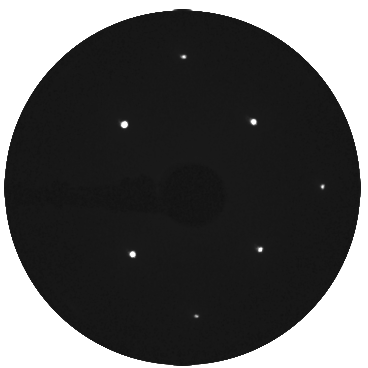
\includegraphics[width=0.25\linewidth]{Plots/LEED_neu/clean_Fe.png}}%
  \qquad
  \subfloat[][]{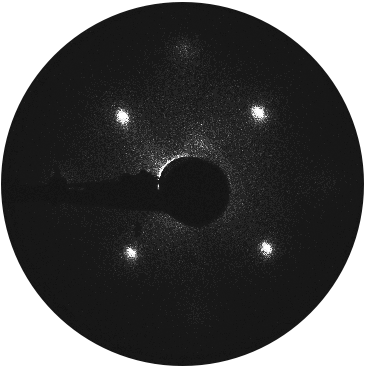
\includegraphics[width=0.25\linewidth]{Plots/LEED_neu/1ML_Fe.png}}%
  \qquad
  \subfloat[][]{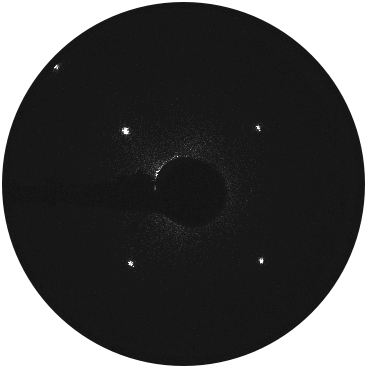
\includegraphics[width=0.25\linewidth]{Plots/LEED_neu/1_6ML_Fe.png}}%
  \qquad
  \subfloat[][]{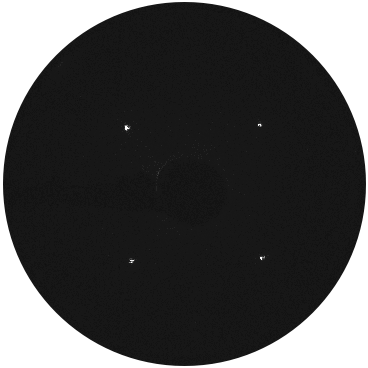
\includegraphics[width=0.25\linewidth]{Plots/LEED_neu/2ML_Fe.png}}%
  \qquad
  \subfloat[][]{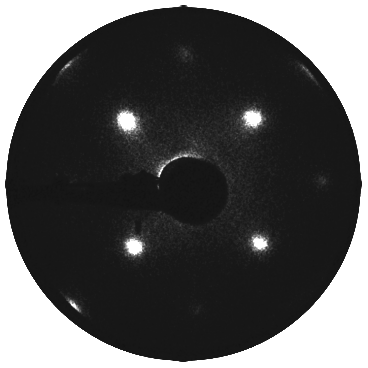
\includegraphics[width=0.25\linewidth]{Plots/LEED_neu/3_5ML_Fe.png}}%
  \qquad
  \subfloat[][]{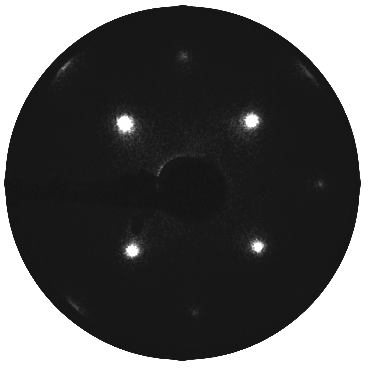
\includegraphics[width=0.25\linewidth]{Plots/LEED_neu/4_3ML_Fe.png}}%
  \caption{LEED-Bilder nach unterschiedlichen Aufdampfdauern von MgO auf Fe(100) bei einer Energie von $E=96\,\si{\eV}$. (a) zeigt sauberes Fe(100),
          (b) eine $1$\,ML Schicht, (c) eine $1,6$\,ML Schicht, (d) eine $2$\,ML Schicht, (e) eine $3,5$\,ML Schicht und (f) eine $4,3$\,ML Schicht.}%
  \label{fig:LEED}
\end{figure}


In Abbildung \ref{fig:LEED} sind auf den LEED-Bildern bei den gleichen Energien $E=96\,\si{\eV}$
die Reflexe bei verschiedenen Schichtdicken von MgO auf reinem Fe(100) zu sehen. 
Die LEED-Bilder können genutzt werden, um eine starke oder schwächere Ordnung der Oberfläche zu 
erkennen und so zum Beispiel zu beurteilen, ob das Wachstum auf der gesamten Probe gleichmäßig verlaufen ist.  
Die unterschiedliche Schärfe der Reflexe ist hier wahrscheinlich auf die unterschiedlichen zugrundeliegenden Wachstumsbedingungen zurückzuführen.



Bei den LEED-Bildern von MgO auf Fe(100)-p(1\,x\,1)O \ref{fig:LEED1}, welche alle im gleichen Wachstumsprozess bei ähnlichen Einstellungen aufgenommen wurden,
ist eine nachlassende Schärfe der Reflexe bei teilweise gefüllten Monolagen zu sehen. 
Bei einer Schichtdicke von $1,1$\,ML liegt eine fast gefüllte ML vor, sodass die Schärfe im Vergleich zur sauberen
Probe etwas nachlässt. Die Reflexe der $2,5$\,ML Schicht sind noch diffuser, 
was sich durch die halbzahlige ML und die dadurch entstehende geringe Ordnung erklären lässt.


%Bei einer Schichtdicke von $1,1$\,ML liegt eine fast gefüllte ML vor,
%die Schärfe lässt im Vergleich zur sauberen Probe etwas nach, 
%bei $2,5$\,ML lässt sie weiter nach, was sich durch die halbzahlige ML und die dadurch entstehende geringe Ordnung erklären lässt.


\begin{figure}[H]
  \centering
  \subfloat[][]{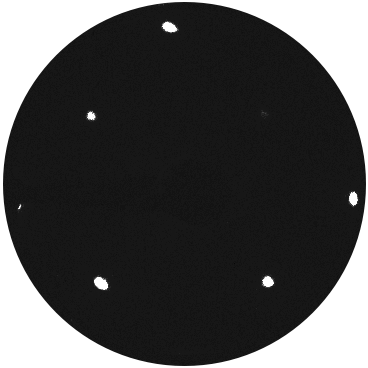
\includegraphics[width=0.25\linewidth]{Plots/LEED_neu/clean_FeO.png}}%
  \qquad
  \subfloat[][]{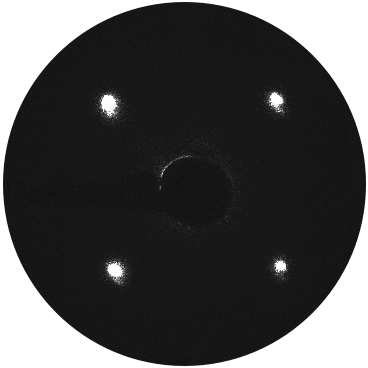
\includegraphics[width=0.25\linewidth]{Plots/LEED_neu/1_1ML_FeO.png}}%
  \qquad
  \subfloat[][]{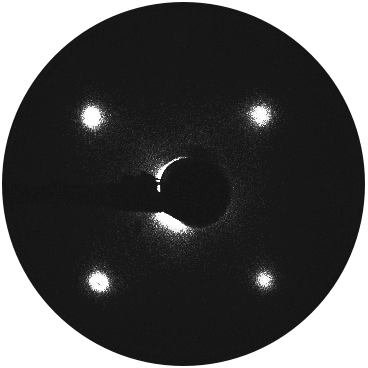
\includegraphics[width=0.25\linewidth]{Plots/LEED_neu/2_5ML_FeO.png}}%

  \caption{LEED-Bilder nach unterschiedlichen Aufdampfdauern von MgO auf Fe(100)-p(1\,x\,1)O bei einer Energie von $E=65\,\si{\eV}$. (a) zeigt die saubere Fe(100)-p(1\,x\,1)O Probe,
          (b) eine $1,1$\,ML Schicht und (c) eine $2,5$\,ML Schicht.}%
  \label{fig:LEED1}
\end{figure}

In Abbildung \ref{fig:LEED2} sind zwei LEED-Bilder von $1,6$\,ML MgO auf reinem Fe(100) zu sehen.
Dabei wurde \ref{fig:LEED2}(a) vor einem schnellen Aufheizen auf $T=600\,\si{\celsius}$ aufgenommen und \ref{fig:LEED2}(b)
danach. Die klareren Reflexe nach dem Aufheizen sprechen für eine bessere Ordnung des Systems.
Dies könnte auf das Entstehen größerer MgO-Domänen hindeuten oder auf das stellenweise Wachstum von Inseln, 
welche durch das Aufheizen aufgebrochen werden.
%was 
%darauf hindeutet, dass Inselstrukturen aufgelöst wurden \ref{sec:Wachstum}. Die  unvollständige Ordnung durch die unbeendete Monolage konnte also 
%durch das Heizen doch noch verbessert werden.

\begin{figure}[H]
  \centering
  \subfloat[][]{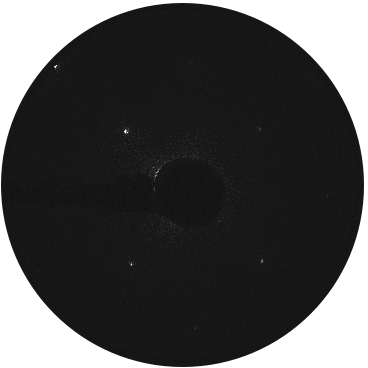
\includegraphics[width=0.25\linewidth]{Plots/LEED_neu/1_6_ML_Fe_96eV_vor_annealen.png}}%
  \qquad
  \subfloat[][]{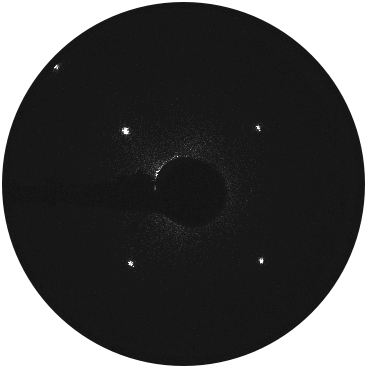
\includegraphics[width=0.25\linewidth]{Plots/LEED_neu/1_6_ML_Fe_96eV_nach_annealen.png}}%
  \caption{LEED-Bilder einer $1,6$\,ML Schicht MgO auf Fe(100) bei einer Energie von $E=96\,\si{\eV}$. (a) zeigt die Probe vor dem Aufheizen,
          (b) zeigt die Probe nach dem Aufheizen.}%
  \label{fig:LEED2}
\end{figure}




\begin{figure}[H]
  \centering
  \begin{subfigure}{0.47\textwidth}
    \includegraphics[width=\textwidth]{Plots/IV-clean_Layout.pdf}
    \caption{}
  \end{subfigure}
  \begin{subfigure}{0.47\textwidth}
    \vspace{-0.2cm}
    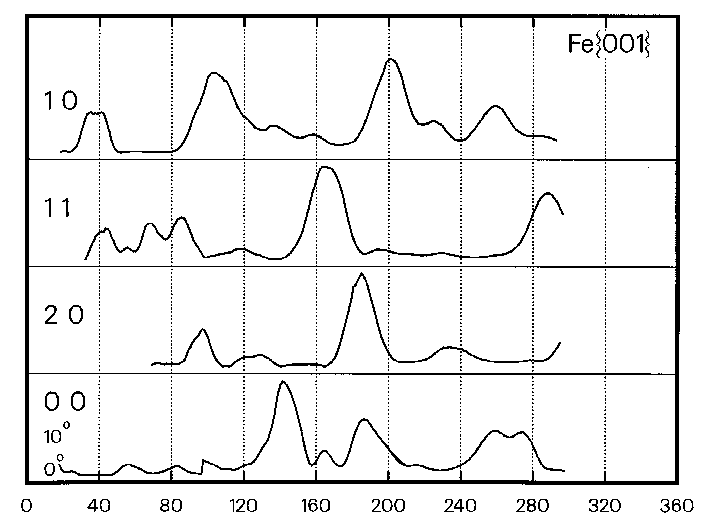
\includegraphics[width=\textwidth]{Plots/fe.png}
    \caption{}
  \end{subfigure}
  \begin{subfigure}{0.47\textwidth}
    \includegraphics[width=\textwidth]{Plots/IV-FeO_Layout.pdf}
    \caption{}
  \end{subfigure}
  \begin{subfigure}{0.47\textwidth}
    \vspace{-0.2cm}
    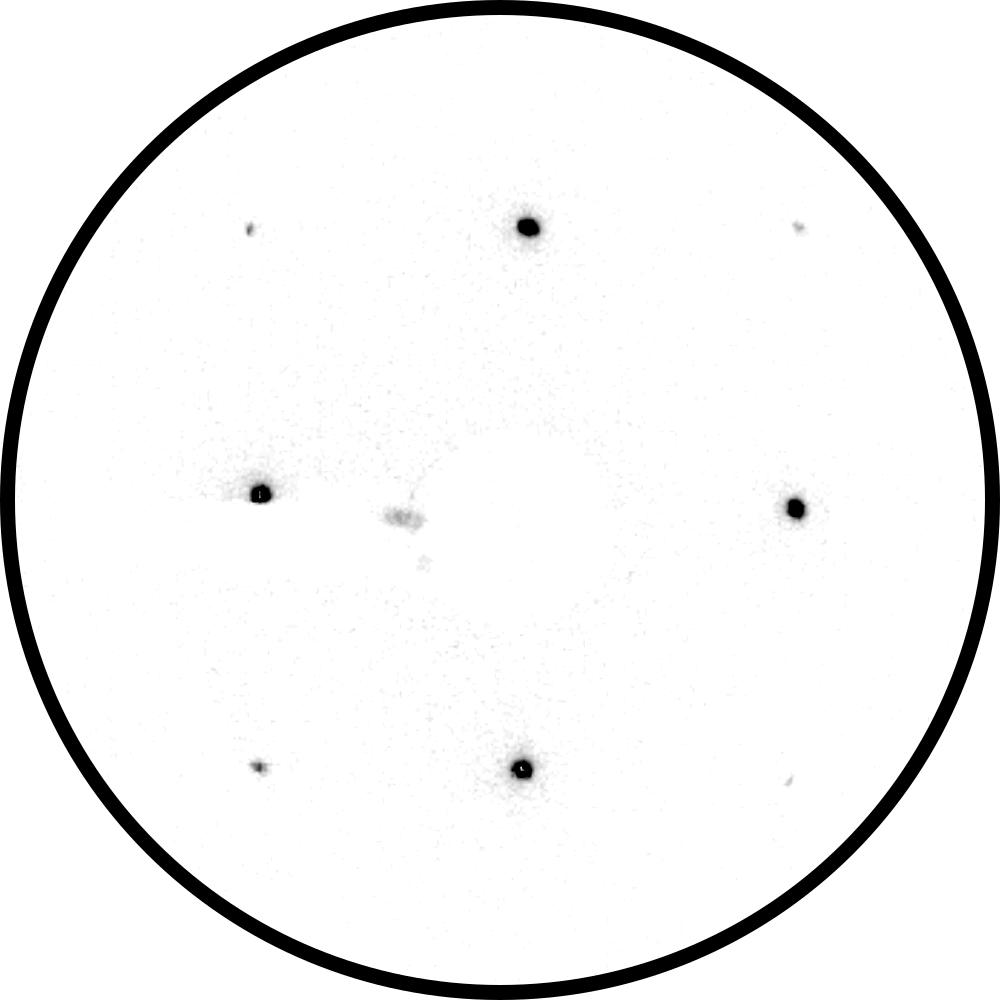
\includegraphics[width=\textwidth]{Plots/feO.png}
    \caption{}
  \end{subfigure}
  \begin{subfigure}{0.47\textwidth}
%    \vspace{-0.2cm}
    \includegraphics[width=\textwidth]{Plots/IV-MgO_Layout.pdf}
    \caption{}
  \end{subfigure}
  \begin{subfigure}{0.47\textwidth}
    \vspace{0.6cm}
    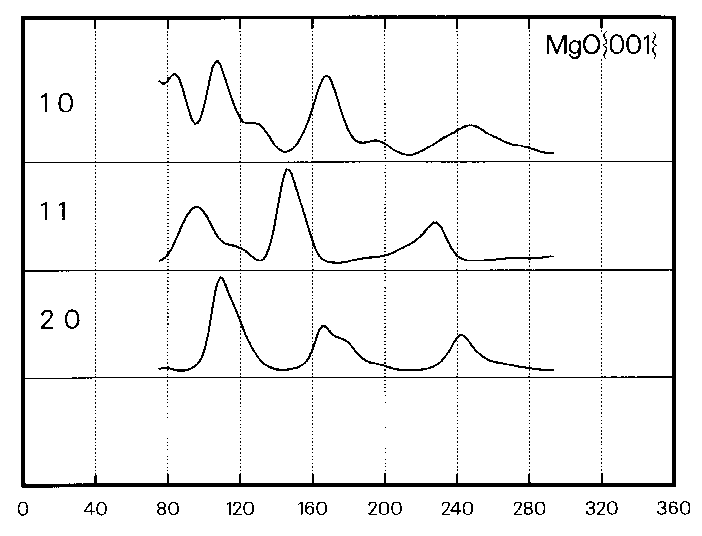
\includegraphics[width=\textwidth]{Plots/mgo.png}
    \caption{}
  \end{subfigure}
  \caption{Aufgenommene IV-Kurven links (a) von sauberem Fe(100), (c) sauberem Fe(100)-p(1\,x\,1)O und (e) MgO. 
          Der (00)-Reflex vom reinen Eisen wurde unter einem $15\,\si{\degree}$ Winkel aufgenommen, der vom passivierten Eisen bei $10\,\si{\degree}$.
          Durch einen Savitzky-Golay Filter 2. Ordnung mit 21 Punkten wurden die
          IV-Kurven geglättet.
          Rechts zum Vergleich Literaturdaten aus dem IV Data Repository \cite{IV}, welche den Daten aus \cite{PhysRevB.16.5271,Legg_1977,JONA1987667,URANO1983109} entsprechen.}%
  \label{fig:IV1}
\end{figure}


Für das reine Eisen, das mit Sauerstoff passivierte Eisen und einen dicken MgO-Film (mehr als 10\,ML)
wurden IV-Kurven aufgenommen. In Abbildung \ref{fig:IV1} ist ein Vergleich der gemessenen Kurven (links) für die 
drei Systeme mit der Literatur (rechts) gezeigt.
Bei dem (10)- und dem (11)-Reflex des passivierten Eisens sind Abweichungen bei den Peakhöhen zu erkennen.
Abgesehen davon liegt eine gute Übereinstimmung der restlichen Reflexe vor.
Die abweichenden Ergebnisse für das passivierte Eisen konnten mehrfach reproduziert werden.


Durch das sukzessive Wachstum ist es möglich, einen zeitlichen Verlauf der IV-Kurven aufzunehmen und Referenzdaten
für eine unterschiedliche Anzahl weniger Monolagen zu erhalten. In Abbildung \ref{fig:IV2} ist eine Zusammenstellung 
dieser IV-Kurven für den (10)-, den (11)- und den (20)-Reflex auf Fe(100) (links) und Fe(100)-p(1\,x\,1)O (rechts) zu sehen.


Die Markierungen zeigen Charakteristika verschiedener Schichtdicken.
Beim MgO-Wachstum auf reinem Eisen ist beim (10)-Reflex in Abbildung \ref{fig:IV2}(a) ein Peak 
bei $240$\,eV bei 1\,ML zu sehen, der bei den anderen vermessenen Schichtdicken nicht auftritt.\newline
Der (11)-Reflex in Abbildung \ref{fig:IV2}(c) zeigt einen Rückgang des $170$\,eV-Peaks vom sauberen Eisen Fe(100), welcher bei 1\,ML kleiner und ab $1,6$\,ML gar nicht mehr sichtbar ist.
Der $140$\,eV-Peak vom MgO-Verlauf ist bereits deutlich ab $1,6$\,ML sichtbar und bleibt bei höheren Schichtdicken konstant.\newline
Ebenso ist der $165$\,eV-Peak des (20)-Reflexes in Abbildung \ref{fig:IV2}(e) von MgO bereits ab $1,6$\,ML zu beobachten, wobei dieser 
bei $1,6$\,ML und $3,5$\,ML noch vom $190$\,eV-Peak überlagert wird. Letzterer nimmt mit zunehmender Schichtdicke an Intensität ab.

Beim MgO-Wachstum auf passiviertem Eisen zeigt der (10)-Reflex in Abbildung \ref{fig:IV2}(b) bereits ab einer Schichtdicke von 1,1\,ML den 
$165$\,eV-Peak von MgO.\newline 
Gleich verhält es sich mit dem $140$\,eV-Peak beim (11)-Reflex in Abbildung \ref{fig:IV2}(d).
Im Vergleich zum Wachstum auf reinem Eisen (siehe Abbildung \ref{fig:IV2}(c)) ist auffällig, dass dieser dort bei einer Schichtdicke von 1\,ML 
noch nicht sichtbar ist.\newline
Ähnlich wie beim (20)-Reflex des Wachstums auf reinem Eisen ist beim (20)-Reflex auf passiviertem Eisen in Abbildung \ref{fig:IV2}(f)
eine Überlagerung zweier Peaks zu sehen. Der $165$\,eV-Peak von MgO überlagert sich ab einer Schichtdicke von 1,1\,ML
mit dem $190$\,eV-Peak, wobei letzterer auch wieder mit steigender Schichtdicke abnimmt.
Wie beim $140$\,eV-Peak beim (11)-Reflex, ist der $190$\,eV-Peak hier beim Wachstum auf reinem Eisen (siehe Abbildung \ref{fig:IV2}(e)) bei einer Schichtdicke von
1\,ML noch nicht sichtbar.

Die aufgeführten Merkmale der IV-Kurven können genutzt werden, um verschiedene Schichtdicken der 
Systeme Fe(100)/MgO und Fe(100)-p(1\,x\,1)O/MgO zu identifizieren.


\begin{figure}[H]
   \centering
   \subfloat[][]{\includegraphics[width=0.47\linewidth]{Plots/IV-10_Layout.pdf}}%
   \qquad
   \subfloat[][]{\includegraphics[width=0.47\linewidth]{Plots/IV-10_FeO-Layout.pdf}}
   \qquad
   \subfloat[][]{\includegraphics[width=0.47\linewidth]{Plots/IV-11_Layout.pdf}}
   \qquad
   \subfloat[][]{\includegraphics[width=0.47\linewidth]{Plots/IV-11_FeO-Layout.pdf}}
   \qquad
   \subfloat[][]{\includegraphics[width=0.47\linewidth]{Plots/IV-20_Layout.pdf}}%
   \qquad
   \subfloat[][]{\includegraphics[width=0.47\linewidth]{Plots/IV-20_FeO-Layout.pdf}}
   \caption{IV-Kurven aufgenommen bei unterschiedlicher Schichtdicke von MgO auf Fe(100) (links) und MgO auf Fe(100)-p(1\,x\,1)O (rechts).
            (a) und (b) zeigen jeweils den (10)-Reflex, (c) und (d) den (11)-Reflex und (e) und (f) den (20)-Reflex.
            Durch einen Savitzky-Golay Filter 2. Ordnung mit 21 Punkten wurden die
          IV-Kurven geglättet.}%
   \label{fig:IV2}
\end{figure}

\chapter{Zusammenfassung und Ausblick}

In dieser Arbeit wurde das Wachstum von MgO sowohl auf Fe(100)- als auch auf Fe(100)-p(1\,x\,1)O-Oberflächen
mit verschiedenen Methoden untersucht. 
Es wurden Daten aufgenommen, die das Wachstum charakterisieren und als mögliche Referenz dienen,
dünne Fe(100)/MgO- und Fe(100)-p(1\,x\,1)O/MgO-Schichtsysteme präzise herzustellen.
%
%Es wurden Referenzdaten dieser Methoden präsentiert, die das Wachstum charakterisieren und  
%somit eine Möglichkeit geben, dünne Fe(100)/MgO- und Fe(100)-p(1\,x\,1)O/MgO-Schichtsysteme präzise zu reproduzieren.

Die Ergebnisse zur Bestimmung der Schichtdicke mittels AES- und MEED-Messungen 
komplementieren sich gegenseitig.
Es hat sich herausgestellt, dass die ersten beiden Monolagen auf Fe(100) schneller 
wachsen und sich anschließend eine Wachstumsrate einstellt, die der konstanten Rate vom Fe(100)-p(1\,x\,1)O/MgO-System entspricht.\newline
Außerdem konnte die für solch ein System charakteristische Abweichung zwischen der ermittelten Wachstumsrate und der 
vorhergesagten QCM-Wachstumsrate bestimmt werden. 

Durch LEED-Aufnahmen vor und nach dem Erhitzen konnte ein positiver Effekt 
des Aufheizens auf die Oberflächenordnung des Fe(100)/MgO-Systems nachgewiesen werden.
Ein Aufbrechen von Inseln bei $1,6$\,ML als Ursache widerspricht den Ergebnissen von Klaua et al. \cite{klaua2001growth} und 
außerdem den Ergebnissen der durchgeführten MEED-Messungen. Als komplementäre Methode zur Untersuchung dieses Effekts 
könnte ein Rastertunnelmikroskop genutzt werden.\newline
Weiterhin wurden charakteristische Merkmale in den IV-Kurven beider Systeme 
für unterschiedliche Schichtdicken herausgearbeitet.

Die Ergebnisse für das geeignete $r/p$-Verhältnis von Tekiel et al. \cite{tekiel2013reactive} konnten nicht bestätigt werden,
denn wie die Elementanalyse mit AES gezeigt hat, entsteht beim Wachstum mehrerer Monolagen ein Sauerstoffüberschuss.\newline
Auffällig ist jedoch, dass die Schichtdickenanalyse mittels AES trotzdem passende Ergebnisse 
sowohl für das Mg/Fe- als auch für das O/Fe-Verhältnis erzeugt hat. 
Weitere Messungen bei verändertem Sauerstoffdruck wären nötig, um dieses Phänomen weiter zu untersuchen. 


Ein hier nicht betrachteter Aspekt ist der gezielte Einbau von Defekten mittels verändertem r/p-Verhältnis 
in der MgO-Schicht. So kann die Austrittsarbeit verändert werden und folglich die Eigenschaften molekularer 
Hybridsysteme gezielt manipuliert werden \cite{greiner2012universal}. 
Notwendig dazu wäre eine Vermessung der Austrittsarbeit zum Beispiel mittels Photoelektronenspektroskopie.
%Ein weiterer Aspekt des Wachstums, der hier nicht betrachtet wurde, ist der gezielte Einbau von Defekten 
%in der MgO-Schicht, um eine Änderung der Austrittsarbeit herbeizuführen.
%Solch eine Veränderung der Austrittsarbeit kann genutzt werden, um die Eigenschaften von molekularen Spinterface-Schichtsystemen 
%gezielt zu manipulieren \cite{greiner2012universal}. \newline
%Gegenstand zukünftiger Untersuchungen könnte also eine Charakterisierung des MgO-Wachstums mit verändertem 
%$r/p$-Verhältnis sein, um gezielt Defekte einzubauen. Damit verbunden wäre eine Vermessung der Austrittsarbeit 
%des Systems zum Beispiel mittels Photoelektronenspektroskopie. 


%Der Einbau solcher Defekte kann durch die hier verwendete Wachstumsmethode durch eine Veränderung des $r/p$-Verhältnises
%vorgenommen werden. Der Versuch das MgO-Wachstum bei Sauerstoffmangel zu charakterisieren ist im Rahmen dieser Arbeit fehlgeschlagen.






%Ein weiterer Effekt, der eine genauere Betrachtung wert ist, ist der Anstieg der MEED-Intensität \ref{fig:MEED1}
%direkt nach dem Öffnen des Shutters. Erwartet wird zunächst eine niedrigere Ordnung der Oberfläche durch das Auftreffen 
%der ersten Fremdatome, welche eine Senkung der Beugungsintensität zur Folge haben sollten.
%Eine solche Senkung ist auch bei den weiteren MEED-Messungen \ref{fig:MEED2} zu erkennen.
%MEED-Messungen unter verschiedenen Bedinungen, vor allem der Variation des Winkels und der vermessenen Beugungsreflexe
%könnten Aufschluss über diesen unerwarteten Effekt bringen.









%\input{content/01_einleitung.tex}
%\chapter{Struktur der Arbeit}

Eine mögliche Struktur der Arbeit sieht wie folgt aus:

\begin{enumerate}
    \item \textbf{Einleitung}\\
        In der \emph{kurzen} Einleitung wird die Motivation für die Arbeit
        dargestellt und ein Einblick in die kommenden Kapitel gegeben.
    \item \textbf{Theoretische Grundlagen}\\
        Alles was an theoretischen Grundlagen benötigt wird, sollte auch eher kurz gehalten werden.
        Statt Grundlagenwissen zu präsentieren, eher auf die entsprechenden Lehrbücher verweisen.
        Etwa: Tiefer gehende Informationen zur klassischen Mechanik entnehmen Sie bitte \cite{kuypers}.
    \item \textbf{Ergebnisse} \\
        Der eigentliche Teil der Arbeit, das was getan wurde.
    \item \textbf{Zusammenfassung und Ausblick} \\
        Zusammenfassung der Ergebnisse, Optimierungsmöglichkeiten, mögliche weitergehende Untersuchungen.
\end{enumerate}

Die Gliederung sollte auf der einen Seite nicht zu fein sein, auf der anderen Seite
sollten sich klar unterscheidende Abschnitte auch kenntlich gemacht werden.

In der hier verwendeten \KOMAScript-Klasse \texttt{scrbook} ist die oberste Gliederungsebene,
die in der Bachelorarbeit verwendet werden sollte, das \texttt{\textbackslash chapter}.

Ein Kapitel sollte erst dann in tiefere Gliederungsebenen unterteilt werden, wenn es auch wirklich etwas zu unterteilen gibt. Es sollte keine Kapitel mit nur einem Unterkapitel (\texttt{\textbackslash section}) geben.

In dieser Vorlage ist die Tiefe des Inhaltsverzeichnisses auf \texttt{chapter} und \texttt{section} beschränkt. Möchten Sie diese Beschränkung aufheben, entfernen Sie den Befehl
\begin{verbatim}
            \setcounter{tocdepth}{1}
\end{verbatim}
aus der Präambel oder ändern Sie den Zahlenwert entsprechend. Das Inhaltsverzeichnis sollte für eine Bachelorarbeit auf eine Seite passen.

%\chapter{Wichtige Hinweise zum Dokument}\label{make}

Diese Vorlage ist auf die Kompilierung mit \texttt{lualatex} ausgelegt. 
Als Dokumentenklasse  wird die \KOMAScript\-Klasse \texttt{scrbook} verwendet.
Falls Sie Änderungen am Layout vornehmen möchten, lesen Sie die \KOMAScript-Dokumentation: \cite{koma}.

Eine umfangreiche Einführung in die moderne Verwendung von \LaTeX{} gibt es hier: \cite{toolbox}, lesenswert ist außerdem das \LaTeX-Tabu: \cite{l2tabu}

Um dieses Dokument vollständig zu erstellen sind maximal vier Programmläufe nötig:
\begin{enumerate}[nosep]
    \item \texttt{lualatex BachelorArbeit.tex}
    \item \texttt{biber BachelorArbeit.bcf}
    \item \texttt{lualatex BachelorArbeit.tex}
    \item \texttt{lualatex BachelorArbeit.tex}
\end{enumerate}

Beim ersten Lauf des \LaTeX-Compilers werden die Kapitel, Links und zitierten Bibliographieeinträge in Hilfsdateien geschrieben.

Dann ist ein Lauf des Programms \texttt{biber} nötig, welches die benötigten Einträge aus der Hilfsdatei einliest, die Einträge aus der \texttt{.bib} Datei einliest, sortiert und formatiert und in eine weitere Hilfsdatei schreibt.

Beim nächsten \LaTeX-Lauf werden dann diese Hilfsdateien eingelesen und Literatur- und Inhaltsverzeichnis erstellt.

Manchmal ist ein vierter Lauf nötig, falls sich durch das einfügen des Literaturverzeichnisses Seitenzahlen verändert haben.

Das Tool \texttt{latexmk} übernimmt dies mit nur einem Programmaufruf und
führ nur so viele Aufrufe durch, wie nötig sind.

\texttt{latexmk --lualatex BachelorArbeit.tex}

Eine gute Option ist es, den \LaTeX{} Output in einem anderen 
Ordner zu erzeugen, dies ist mit der \texttt{--output-directory} Option möglich:

\texttt{latexmk --output-directory=build --lualatex BachelorArbeit.tex}


\section{Erstellen des Ausgabedokuments mit Make}

Für diese Vorlage wird ein Makefile zur Verfügung gestellt, welches automatisch alle Schritte ausführt, die für das fertige Dokument nötig sind.
Die Ausgabe erfolgt dabei in den Unterordner \texttt{build/}.
Make prüft, ob die Quelldateien verändert wurden, falls nicht, werden auch keine Befehle ausgeführt.

Falls Sie das Makefile benutzen möchten, sollten Sie alle Abhängigkeiten eintragen (Eigene Dateien für Kapitel, Plots, etc.).


Download und weitere Informationen zu Make gibt es unter \cite{make}. Die Befehle sind für die Bash ausgelegt.
Wenn Sie sie unter Windows nutzen wollen, benötigen Sie einen Bash-Emulator, wie Git Bash, Download unter \cite{gitbash} möglich.
Wenn Sie Make installiert haben, rufen Sie einfach in der Konsole im Verzeichnis der Arbeit den Befehl \texttt{make}.

\section{Erstellen des Ausgabedokuments mit Texmaker}
\subsection{Einrichten der nötigen Befehle}
Ein beliebter Editor für alle Betriebssysteme ist Texmaker, Download unter \cite{texmaker}.
Damit Texmaker das Dokument korrekt kompiliert, fügen sie einen benutzerdefinierten Befehl hinzu:
\begin{enumerate}[nosep]
    \item Klicken sie oben in der Menüleiste auf \emph{Benutzer/in}
    \item Klick auf \emph{Eigene Befehle}
    \item Klich auf \emph{Eigene Befehle editieren}, dort können Sie bis zu 5 eigene Befehle definieren
    \item Geben Sie dem Befehl unter \emph{Menüeintrag} einen Namen und tragen sie folgende Befehle in das Befehlsfeld ein: \\
      \small\verb+latexmk --lualatex --interaction=batchmode --halt-on-error %.tex |+
    \item Bestätigen Sie mit \emph{OK}
\end{enumerate}

\begin{figure}
    \centering
    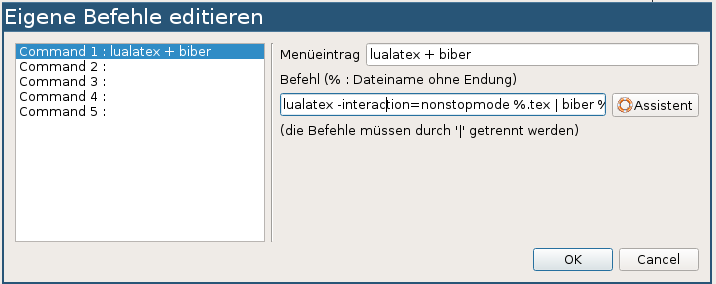
\includegraphics[width=12cm]{Plots/texmaker.png}
    \caption{Screenshot zur Erstellung des Kompilier-Befehls in Texmaker}
    \label{fig:texmaker}
\end{figure}


In Abbildung \ref{fig:texmaker} ist ein Screenshot des Befehlsmenü gezeigt. Ihren Befehl können Sie nun im Drop-Down-Menü zum 
Kompilieren des Dokuments auswählen und mit einem Klick auf den Pfeil starten.

\subsection{Aufräumen}

Nach einem \LaTeX-Fehler ist es oft notwendig, die erstellten Hilfsdateien zu löschen.
Klicken Sie hierzu auf \emph{Werkzeuge}→\emph{Aufräumen}.


\chapter{\LaTeX-Grundlagen}

Bitte beachten Sie beim Schreiben der Arbeit folgende Konventionen bzw. Grundlagen:

\begin{itemize}
    \item \textbf{Abschnitte und Zeilenumbrüche} \\
        Es sollten im Fließtext keine Zeilenumbrüche mit \textbackslash\textbackslash \ erzwungen werden.
        Schreiben Sie höchsten einen Satz in eine Code-Zeile.
        Absätze werden im Code mit einer Leerzeile markiert und dann entsprechend der Einstellung von \texttt{parskip} in der Dokumentenklasse gesetzt.
    \item \textbf{Kursiv/Aufrecht} \\
        \begin{itemize}
            \item Variablen und physikalische Größen werden kursiv gesetzt. 
            \item Einheiten werden immer aufrecht und mit einem halben Leerzeichen Abstand zur Zahl gesetzt. Nutzen Sie \texttt{siunitx}!
            \item Mathematische Konstanten und Funktionen werden ebenfalls aufrecht gesetzt. Zum Beispiel die Eulersche Zahl e, das imaginäre i und das infinitesimale d.
                Im Mathematikmodus können Sie dies mit dem Befehl \verb_\mathrm{}_ erreichen. Für die Funktionen stellt \LaTeX \ Befehle bereit, z.B. \verb+\arccos+.
            \item Integrand und ein $\mathrm{d}x$ sollten ebenfalls durch ein kleines Leerzeichen (\verb+\,+) getrennt werden.
        \end{itemize}
        


\end{itemize}

\section{Zahlen und Einheiten}

Jede Zahl, jede Einheit und jede Zahl mit Einheit sollte mit Hilfe der in dem Paket \texttt{siunitx} zur Verfügung gestellten Befehle gesetzt werden.
Grundsätzlich gilt: Einheiten werden aufrecht gesetzt und haben ein kleines Leerzeichen (\verb+\,+) Abstand zu ihrer Zahl. 
Werden Fließkommazahlen ohne \texttt{siunitx} gesetzt, entsteht ein hässlicher Leerraum zwischen Komma und erster Nachkommastelle, da \LaTeX \ das Komma nicht als Dezimaltrennzeichen, sondern als Satzzeichen interpretiert.

Das Paket wurde mit deutschen Spracheinstellungen (also mit Komma als Dezimaltrennzeichen und $\cdot$ zwischen Zahl und Zehnerpotenz) geladen, sowie mit den Einstellungen, dass die Standardabweichung stets durch $\pm$ abgetrennt wird und Einheiten falls nötig als Brüche ausgegeben werden.

\begin{table}
    \centering
    \caption{Beispiele für siunitx}
    \label{tab:si}
    \begin{tabular}{l r}
        \toprule
        Befehl     &   Ergebnis \\
        \midrule
        \verb+\num{1.2345}+ & \num{1.2345} \\
        \verb+\num{1.2e3}+ & \num{1.2e3} \\
        \verb_\num{1.2 +- 0.2}_ & \num{1.2+-0.2} \\
        \verb+\num{10000}+ & \num{10000} \\
        \verb+\si{\meter\per\second}+ & \si{\meter\per\second} \\
        \verb+\SI{1.2(1)}{\micro\ampere}+ & \SI{1.2(1)}{\micro\ampere} \\
        \verb+\SI{1.2\pm0.1e3}{\kilo\gram\per\cubic\meter}+ & \SI{1.2\pm0.1e3}{\kilo\gram\per\cubic\meter} \\
        \bottomrule 
    \end{tabular}
\end{table}

Das Paket stellt unter anderem die drei wichtigen Befehle
\begin{itemize}
    \item \texttt{\textbackslash num\{Zahl\}},
    \item \texttt{\textbackslash si\{Einheit\}} und
    \item \texttt{\textbackslash SI\{Zahl\}\{Einheit\}}
\end{itemize}
zur Verfügung.
Diese Befehle sollten stets genutzt werden, wenn Zahlen angegeben werden. 
Sie funktionieren sowohl im Text- als auch im Mathematikmodus.
In Tabelle \ref{tab:si} sind einige Beispiele aufgetragen. Bitte lesen Sie die Dokumentation \cite{siunitx}.

\section{Das Literaturverzeichnis}

Das Literaturverzeichnis wird mit Hilfe von BibLaTeX und biber erstellt.
Tragen Sie alle ihre Quellen in die Datei \texttt{references.bib} ein, Sie enthält bereits
einige Beispiele. Für weitere Informationen lesen Sie bitte die Dokumentation \cite{biblatex}.

Im Text können Sie mit \verb_\cite{kürzel}_ zitieren. Seitenzahlen geben Sie in eckigen Klammern an:
\verb_\cite[10]{kürzel}_. 

Das Literaturverzeichnis ist so eingestellt, dass es Ihre Quellen in alphabetischer Reihenfolge nach Autoren nummeriert.
Möchten Sie das Literaturverzeichnis nach der Reihenfolge des Auftauchens im Text sortieren, fügen sie die Paktetoption \texttt{sorting=none} beim Laden
des BibLaTeX-Pakets hinzu.

Den Zitier- und Bibliographie-Stil geben sie mit der Option \texttt{style=Stil} an. Die beiden gebräuchlisten Stile sind \texttt{numeric} und \texttt{alphabetic}. 
Bei \texttt{numeric} werden die Quellen durchnummeriert, bei \texttt{alphabetic} wird ein Buchstabenkürzel aus Autor(en)-Name(n) und Jahr verwendet.
Für weitere Stile konsultieren Sie bitte die Dokumentation: \cite{biblatex}.

Ein Beispiel für das Zitieren eines Buches lautet so \cite{handbook_adhesives},
wissenschaftliche Artikel hingegen werden so \cite{einstein} zitiert.

Damit das Literaturverzeichnis erstellt wird, ist ein Aufruf von \texttt{biber} nach einem ersten kompilieren mit \texttt{lualatex} nötig.
Danach muss das Dokument erneut mit \texttt{lualatex} kompiliert werden. 

Zum korrekten Kompilieren des Dokuments siehe Kapitel \ref{make}.

%\chapter{Abbildungen und Tabellen}

\section{Abbildungen}

Achten Sie bei ihren Plots auf ausreichend große Achsenbschriftungen, ausreichende Schriftdicken und gut unterscheidbare Farben.
Im Idealfall haben Sie im Plot und der Arbeit die gleiche Schriftgröße und Schriftart.
Dies lässt sich durch Erstellen des Plots in der korrekten Größe und Einbinden mit dem optionalen Argument \texttt{scale=1} erreichen. Ein Beispiel sehen Sie in Abbildung \ref{fig:bsp}.

Nutzen Sie wenn möglich Vektorgrafiken (pdf) und nur in Ausnahmen Rastergrafiken wie .png oder .jpg.
Setzen Sie Punkte hinter Abbildungsunterschriften.

\begin{figure}
    \centering
    \includegraphics[scale=1]{./Plots/Histogramm.pdf}
    \caption{Ein Histogramm mit Fehlerbalken für zwei Datensätze, Schriftgröße und -art entsprechen der des Dokuments.}
    \label{fig:bsp}
\end{figure}

\section{Tabellen}

Tabellen sollten so einfach wie möglich aufgebaut sein, verzichten Sie auf zu viele Linien. In fast allen Fällen reichen drei horizontale Linien aus, jeweils über und unter der Tabelle und zwischen den Spaltenüberschriften und der eigentlichen Tabelle.

Das Paket \texttt{booktabs} stellt hierfür \verb_\toprule_, \verb_\midrule_ und 
\verb_\bottomrule_ zur Verfügung.
Das Paket \texttt{siunitx} stellt eine extrem mächtige neue Spalteneinstellung bereit: \texttt{S}, mit ihr können Zahlen und Einheiten sehr sauber und gut ausgerichtet gesetzt werden.

Diese Vorlage geht von Tabellenüberschriften aus, möchten Sie dagegen Tabellenunterschriften entfernen Sie das entsprechende optionale Argument für die Dokumentenklasse in der Präambel.

Ein Beispiel ist Tabelle~\ref{tab:bsp}.
\begin{table}
    \centering
    \caption{Beispieltabelle mit willkürlichen Werten, für die Zahlenwerte wurde die S-Option aus \texttt{siunitx} verwendet.}
    \label{tab:bsp}
    \begin{tabular}{S[table-format=4.2] S[table-format=3.2]}
        \toprule
        {$p \mathrel{/} \si{\pascal}$}  & {$T \mathrel{/} \si{\kelvin}$} \\
        \midrule
        1024,23 & 273,15 \\
        1025,31 & 274,5 \\
        1026,27 & 276,2 \\
        \bottomrule
    \end{tabular}
\end{table}


\appendix
% Hier beginnt der Anhang, nummeriert in lateinischen Buchstaben
%\chapter{Ein Anhangskapitel}

Hier könnte ein Anhang stehen, falls Sie z.\,B.\ Code, Konstruktionszeichnungen oder Ähnliches mit in die Arbeit bringen wollen.
Im Normalfall stehen jedoch alle Ihre Resultate im Hauptteil der Bachelorarbeit und ein Anhang ist überflüssig.

\backmatter
\printbibliography
%\chapter*{Acknowledgement}
\section*{Acknowledgement}
\markleft{Danksagung}
I would like to thank all the people, without whom this thesis would not have been possible.
%
%Schließlich möchte ich all denen danken, ohne die 
%diese Arbeit nicht möglich gewesen wäre.

I am very grateful towards Prof. Mirko Cinchetti for arousing my interest in solid-state physics
and giving me the opportunity to write this thesis at his research group.

%Zunächst danke ich Prof. Mirko Cinchetti dafür, dass 
%er bei mir das Interesse an der Festkörperphysik geweckt hat und es mir ermöglichte,  
%diese Arbeit an seinem Lehrstuhl zu schreiben.
%
Furthermore I would like to thank my supervisors Dr. Giovanni Zamborlini and David Janas
for the huge help in all stages of this thesis, like the introduction
to the laboratory work and the discussion of the experimental results.

And finally I would also like to thank the whole
Experimental Physics 6 group for the great 
work atmosphere and for taking time
to discuss my questions.

\cleardoublepage
\includepdf{Plots/scan0004}
%\thispagestyle{empty}
\section*{Eidesstattliche Versicherung}
Ich versichere hiermit an Eides statt, dass ich die vorliegende Abschlussarbeit mit dem Titel \enquote{\thetitle} selbstständig und ohne unzulässige fremde Hilfe erbracht habe.
Ich habe keine anderen als die angegebenen Quellen und Hilfsmittel benutzt, sowie wörtliche und sinngemäße Zitate kenntlich gemacht. 
Die Arbeit hat in gleicher oder ähnlicher Form noch keiner Prüfungsbehörde vorgelegen.

\vspace*{1cm}\noindent
\begin{center}
  \begin{tabular}{@{}p{0.4\textwidth}@{\hspace{0.15\textwidth}}p{0.4\textwidth}@{}}
  \rule{\linewidth}{0.25pt}& \rule{\linewidth}{0.25pt}\\
  Ort, Datum & Unterschrift
  \end{tabular}
\end{center}

\subsection*{Belehrung}
Wer vorsätzlich gegen eine die Täuschung über Prüfungsleistungen betreffende Regelung einer Hochschulprüfungsordnung verstößt, handelt ordnungswidrig.
Die Ordnungswidrigkeit kann mit einer Geldbuße von bis zu \SI[round-mode=places, round-precision=2]{50000}{€} geahndet werden. 
Zuständige Verwaltungsbehörde für die Verfolgung und Ahndung von Ordnungswidrigkeiten ist der Kanzler/die Kanzlerin der Technischen Universität Dortmund. 
Im Falle eines mehrfachen oder sonstigen schwerwiegenden Täuschungsversuches kann der Prüfling zudem exmatrikuliert werden \mbox{(\S\,63 Abs. 5 Hochschulgesetz --HG--).}

Die Abgabe einer falschen Versicherung an Eides statt wird mit Freiheitsstrafe bis zu 3 Jahren oder mit Geldstrafe bestraft.

Die Technische Universität Dortmund wird ggf.\ elektronische Vergleichswerkzeuge (wie z.\,B.\ die Software \enquote{turnitin}) zur Überprüfung von Ordnungswidrigkeiten in Prüfungsverfahren nutzen. \\[\baselineskip]

\noindent Die oben stehende Belehrung habe ich zur Kenntnis genommen.\\[1cm]
\begin{center}
\begin{tabular}{@{}p{0.4\textwidth}@{\hspace{0.15\textwidth}}p{0.4\textwidth}@{}}
\rule{\linewidth}{0.25pt}& \rule{\linewidth}{0.25pt}\\
Ort, Datum & Unterschrift
\end{tabular}
\end{center}

\end{document}
